% 设置正文字体为小四号宋体(12pt对应小四号)
\documentclass[oneside,12pt,reqno]{ctexart}
% ctexart默认使用宋体,12pt对应小四号
%---------------------------------------------------------------------------%
%-                                Packages                                 -%
%---------------------------------------------------------------------------%
% ctex + xeCJK 环境下不再需要 CJK 宏包(避免与 xeCJK 冲突)
% \usepackage{CJK,CJKnumb}
\usepackage{url}
% 正文引用只显示文献编号,右上角上标;参考文献表仍按 GB/T 7714-2015 格式
\usepackage[backend=biber,sorting=none,gbpub=false,bibstyle=gb7714-2015,citestyle=numeric,
gbpunctin=false,gbnamefmt=lowercase,
]{biblatex}
% 引用为正文内 [x] 格式(如 [1] [2]),非上标;仅输出编号,避免 gb7714-2015 输出作者名
\DeclareCiteCommand{\cite}[\mkbibbrackets]
  {\usebibmacro{citeindex}}
  {\usebibmacro{citeindex}%
   \printfield{labelnumber}}
  {\multicitedelim}
  {}
\providecommand*{\mkbibbrackets}[1]{[#1]}

\usepackage{amsmath, amsfonts, amssymb}
\usepackage{booktabs}
\usepackage{fontspec}
\usepackage{threeparttable}
\usepackage{multicol}
\usepackage{multirow}
\usepackage{fancyhdr}
\usepackage{latexsym}
\usepackage{mathrsfs}
% \usepackage{wasysym}  % 字体文件缺失,暂时注释
\usepackage{enumerate}
\usepackage{titletoc}
\usepackage{titlesec}
% 设置章节标题到页眉
\makeatletter
\renewcommand{\sectionmark}[1]{\markboth{#1}{}}
\newcommand{\StartToc}[1]{\@starttoc{#1}}
\let\saved@numberline\numberline
\makeatother

\newlength{\titlelabelsep}
\setlength{\titlelabelsep}{1em}

% 一级标题(章):三号黑体,水平居中,段前段后正常
\titleformat{\section}
  {\normalfont\sanhao\bfseries\heiti\centering}
  {}                                  % 编号由标题文字自带(如“第一章”),不重复输出
  {0pt}
  {}
\titleformat{name=\section,numberless}
  {\normalfont\sanhao\bfseries\heiti\centering}
  {}
  {0pt}
  {}
\titlespacing*{\section}{0pt}{\baselineskip}{0.5\baselineskip}

% 二级标题(节):黑体四号,居左,段前段后正常
\titleformat{\subsection}
  {\normalfont\sihao\bfseries\heiti}
  {\thesubsection}
  {\titlelabelsep}
  {}
\titleformat{name=\subsection,numberless}
  {\normalfont\sihao\bfseries\heiti}
  {}
  {0pt}
  {}
% 标题前后间距(按需更紧凑)
\titlespacing*{\subsection}{0pt}{0.6\baselineskip}{0.25\baselineskip}

% 三级标题(条):小四黑体,居左,无额外段落间距
\titleformat{\subsubsection}
  {\normalfont\xiaosihao\bfseries\heiti}
  {\thesubsubsection}
  {\titlelabelsep}
  {}
\titleformat{name=\subsubsection,numberless}
  {\normalfont\xiaosihao\bfseries\heiti}
  {}
  {0pt}
  {}
\titlespacing*{\subsubsection}{0pt}{0.35\baselineskip}{0.15\baselineskip}
\usepackage{epstopdf}
\usepackage{caption}
\usepackage{graphicx, subfig}
\usepackage{float}
\floatplacement{figure}{H}
\floatplacement{table}{H}
\usepackage{fancyhdr} 
% 页面设置已在 main.tex 中统一设置,此处删除避免冲突
%---------------------------------------------------------------------------%
%-                                  Fonts                                  -%
%---------------------------------------------------------------------------%
\newcommand{\song}{\CJKfamily{song}}    % 宋体   (simsun.ttf)
\makeatletter
\@ifundefined{songti}{\newcommand{\songti}{\CJKfamily{song}}}{}
\@ifundefined{heiti}{\newcommand{\heiti}{\CJKfamily{hei}}}{}
\makeatother
\newcommand{\fs}{\CJKfamily{fs}}        %仿宋体  (simfs.ttf)
\newcommand{\kai}{\CJKfamily{kai}}      % 楷体   (simkai.ttf)
\newcommand{\hei}{\CJKfamily{hei}}      % 黑体   (simhei.ttf)
\newcommand{\li}{\CJKfamily{li}}        % 隶书   (simli.ttf)
%---------------------------------------------------------------------------%
%-                                  Sizes                                  -%
%---------------------------------------------------------------------------%
\newcommand{\chuhao}{\fontsize{42pt}{\baselineskip}\selectfont}
\newcommand{\xiaochuhao}{\fontsize{36pt}{\baselineskip}\selectfont}
\newcommand{\yihao}{\fontsize{28pt}{\baselineskip}\selectfont}
\newcommand{\erhao}{\fontsize{21pt}{\baselineskip}\selectfont}
\newcommand{\xiaoerhao}{\fontsize{18pt}{\baselineskip}\selectfont}
\newcommand{\sanhao}{\fontsize{16pt}{18pt}\selectfont}   % 三号,标题用
\newcommand{\sihao}{\fontsize{14pt}{\baselineskip}\selectfont}
\newcommand{\xiaosihao}{\fontsize{12pt}{14.4pt}\selectfont} % 小四,标题用
\newcommand{\wuhao}{\fontsize{10.5pt}{\baselineskip}\selectfont}
\newcommand{\xiaowuhao}{\fontsize{9pt}{\baselineskip}\selectfont}
\newcommand{\liuhao}{\fontsize{7.875pt}{\baselineskip}\selectfont}
\newcommand{\qihao}{\fontsize{5.25pt}{\baselineskip}\selectfont}
%---------------------------------------------------------------------------%
%-                               Chinesization                             -%
%---------------------------------------------------------------------------%
\newtheorem{theorem}{\hskip 2em定理}[section]
\newtheorem{definition}{\hskip 2em定义}[section]
\newtheorem{exam}{\hskip 2em例}[section]
\newtheorem{proof}{{\it \hskip 2em\textbf{证明}}}
\newtheorem{solution}{{\it \hskip 2em\textbf{解}}}
\renewcommand{\tablename}{\songti 表}
\renewcommand{\figurename}{\song 图}
\renewcommand{\refname}{\centerline {参考文献}}
% 目录、图目录、表目录标题:黑体三号,居中
\renewcommand{\contentsname}{\centerline{\sanhao\heiti 目~~~~录}}
\renewcommand{\listfigurename}{\centerline{\sanhao\heiti 图~~~~目~~~~录}}
\renewcommand{\listtablename}{\centerline{\sanhao\heiti 表~~~~目~~~~录}}
\renewcommand{\thefootnote}{\arabic{footnote}}
\renewcommand{\theequation}{\thesection.\arabic{equation}}
% 图表编号格式:按章编号,使用短横线(如"图3-1"、"表2-1")
\renewcommand{\thefigure}{\thesection-\arabic{figure}}
\renewcommand{\thetable}{\thesection-\arabic{table}}
%---------------------------------------------------------------------------%
%-                                公式随章编号                               -%
%---------------------------------------------------------------------------%
\date{}
\makeatletter
\renewcommand*\l@chapter[2]{%
 \ifnum \c@tocdepth >\m@ne
   \addpenalty{-\@highpenalty}%
   \vskip 0.4em \@plus\p@
   \setlength\@tempdima{0em}%
   \begingroup
     \parindent \z@ \rightskip \@pnumwidth
     \parfillskip -\@pnumwidth
     \leavevmode \bfseries
     \advance\leftskip\@tempdima
     #1\nobreak\leaders\hbox{$\m@th
       \mkern \@dotsep mu\hbox{.}\mkern \@dotsep
       mu$}\hfill \nobreak\hb@xt@\@pnumwidth{\hss #2}\par
     \penalty\@highpenalty
   \endgroup
 \fi}
\date{}
\numberwithin{equation}{section}
\numberwithin{figure}{section}
\numberwithin{table}{section}
%---------------------------------------------------------------------------%
%-                              Tabular Option                             -%
%---------------------------------------------------------------------------%
\newcommand{\tabincell}[2]{\begin{tabular}{@{}#1@{}}#2\end{tabular}}
%---------------------------------------------------------------------------%
%-                              Caption Option                             -%
%---------------------------------------------------------------------------%
% 图表标题格式:五号宋体,紧凑间距
\DeclareCaptionFont{nwucaption}{\wuhao\songti}
\captionsetup[figure]{labelsep=space,font={nwucaption},skip=3pt,belowskip=3pt}
\captionsetup[table]{labelsep=space,font={nwucaption},skip=3pt,aboveskip=3pt}
% 减少图表与正文的间距
\setlength{\floatsep}{6pt plus 2pt minus 2pt}      % 两个浮动体之间的距离
\setlength{\textfloatsep}{8pt plus 2pt minus 2pt}  % 浮动体与正文之间的距离
\setlength{\intextsep}{6pt plus 2pt minus 2pt}     % 浮动体在文本中的间距
%---------------------------------------------------------------------------%
%-                             Reference Resource                          -%
%---------------------------------------------------------------------------%
% \addbibresource{Tex/reference.bib}  % 已在 main.tex 中配置
%---------------------------------------------------------------------------%
%-                                Page Control                             -%
%---------------------------------------------------------------------------%
% 版心由 main.tex 中 \geometry 统一设置,此处不再重复以免冲突
% 目录格式:符合中文学术论文标准
% 目录标题:居中,三号黑体(已在上面设置 \contentsname)

% 第一级(章):黑体四号字,顶格;不显示章前数字(仅显示“第一章”“第二章”等标题文字)
\titlecontents{section}[0em]{\fontsize{14pt}{16.8pt}\selectfont\heiti\bfseries\renewcommand{\numberline}[1]{}}{}{}%
{\titlerule*[0.7pc]{$\cdot$}\contentspage}[\vspace{0.5pt}\let\numberline\saved@numberline]

% 第二级(节):宋体小四号字,缩进 2.5em(1.1 等靠后)
\titlecontents{subsection}[2.5em]{\fontsize{12pt}{14.4pt}\selectfont\songti}{\contentslabel{2.5em}\ }%
{}{\titlerule*[0.7pc]{$\cdot$}\contentspage}[\vspace{0.5pt}]

% 第三级(条):宋体小四号字,缩进 3.8em(相对节再靠后)
\titlecontents{subsubsection}[3.8em]{\fontsize{12pt}{14.4pt}\selectfont\songti}{\contentslabel{3em}\ }%
{}{\titlerule*[0.7pc]{$\cdot$}\contentspage}[\vspace{0.5pt}]

% 第四级(段):宋体小四号字,缩进 4em
\titlecontents{paragraph}[4em]{\fontsize{12pt}{14.4pt}\selectfont\songti}{\contentslabel{3.5em}\ }%
{}{\titlerule*[0.7pc]{$\cdot$}\contentspage}[\vspace{0.5pt}]
% 图目录和表目录格式:五号宋体,紧凑间距,与目录格式一致
\makeatletter
\renewcommand*\l@figure{\@dottedtocline{1}{0em}{2.3em}}
\renewcommand*\l@table{\@dottedtocline{1}{0em}{2.3em}}
\makeatother
\renewcommand{\baselinestretch}{1.5}  % 正文行间距1.5倍,符合格式要求
% 设置段落首行缩进
\usepackage{indentfirst}  % 确保每个段落首行都缩进
\setlength{\parindent}{2em}  % 每个段落首行缩进2个字符
\renewcommand{\textfraction}{0.15}    % 正文至少占页面的15%(避免图片占满整页)
% \renewcommand{\floatpagefraction}{0.8}% 图片占页面80%以上才会单独占页
\renewcommand{\topfraction}{0.85}     % 顶部浮动体最多占页面85%
\renewcommand{\bottomfraction}{0.85}

\addbibresource{chapters/reference.bib}

% --- 1. 基础宏包 ---
\usepackage{amsmath, amssymb, amsfonts} % 数学公式 (去重)
\usepackage{indentfirst}
\usepackage{graphicx}   % 图片
\usepackage{booktabs}   % 三线表
\usepackage{geometry}   % 页面设置
\usepackage{fancyhdr}   % 页眉页脚
\usepackage{hyperref}   % 超链接
\usepackage{titletoc}   % 目录格式
\usepackage{enumitem}
\usepackage{algorithm}    % 算法浮动环境
\usepackage{algorithmicx} % 算法结构扩展
\usepackage{algpseudocode}% 算法关键词(For/If/State等)
\usepackage{amsmath}      % 数学公式支持
\usepackage{amssymb}
% 注意:参考文献使用 biblatex(在 option.tex 中已配置),不需要 natbib

% --- 2. 算法宏包 (修复冲突) ---
\usepackage{algorithm}  
\usepackage{algpseudocode} % 推荐使用这个现代包
% \usepackage{algorithmic} % 已注释:与 algpseudocode 冲突,建议不用


% --- 3. 页面设置 (参考西北大学标准) ---
% 版心仅由此处 geometry 统一设置,option.tex 中不再重复以免冲突
\geometry{left=3cm, right=2.5cm, top=3cm, bottom=2.5cm}
\setlength{\headheight}{14.5pt}  % 消除 fancyhdr 页眉高度过小警告

% --- 4. 页眉页脚设置 ---
% 页眉统一:宋体五号(10.5pt),水平居中(目录、图目录、表目录等均同)
\newcommand{\headerfont}{\wuhao\songti}
\pagestyle{fancy}
\fancyhf{}
\fancyhead[C]{\headerfont\leftmark}
\renewcommand{\headrulewidth}{0.4pt}
\fancyfoot[C]{\small \thepage}
% plain 样式同样使用宋体五号页眉
\fancypagestyle{plain}{%
  \fancyhf{}
  \fancyhead[C]{\headerfont\leftmark}
  \renewcommand{\headrulewidth}{0.4pt}
  \fancyfoot[C]{\small \thepage}
}
% 每章结束后留一页空页
\newcommand{\chapterblank}{\clearpage\thispagestyle{empty}\null\newpage}
% ctexart 无 \mainmatter,定义为空操作以免报错
\providecommand{\mainmatter}{}

% --- 信息录入 ---
\title{基于对比学习的联邦异构图推荐算法与系统研究}
\author{伍勋高}
\date{2025年6月}

\begin{document}
\let\maketitle\relax  % 不输出标题页,避免摘要前出现 *、[1]¹ 等


% =========================================================
%   前置部分 (Front Matter)
%   特点:页码为罗马数字 (i, ii, iii...);不用 \frontmatter 避免摘要前出现多余空白与符号
% =========================================================
% \frontmatter  % 已注释:避免首页出现 * [1]1 等

% 1. 封面页(已删除)
% % 封面页
% 如果需要自定义封面,可以在这里添加内容
% 当前使用默认的 \maketitle
% 注意:这是一个子文件,需要从 main.tex 中 \input 使用

\maketitle
\thispagestyle{empty}
\newpage





% 2. 声明页 (独创性声明)(已删除)
% % 独创性声明页
% 注意:这是一个子文件,需要从 main.tex 中 \input 使用

\newpage
\thispagestyle{empty}

\begin{center}
    \Large\textbf{独创性声明}
\end{center}

\vspace{2cm}

本人声明所呈交的学位论文是本人在导师指导下进行的研究工作及取得的研究成果。据我所知,除了文中特别加以标注和致谢的地方外,论文中不包含其他人已经发表或撰写过的研究成果,也不包含为获得西北大学或其他教育机构的学位或证书而使用过的材料。与我一同工作的同志对本研究所做的任何贡献均已在论文中作了明确的说明并表示谢意。

\vspace{3cm}

\begin{flushright}
    学位论文作者签名:\underline{\hspace{3cm}} \hspace{2cm} 日期:\underline{\hspace{3cm}}
\end{flushright}

\newpage





% 3. 摘要页 (中英文摘要)
% --- 摘要页设置开始(不另起页,避免首页空白) ---
\pagenumbering{Roman} % 设置页码为罗马数字 I, II, III
\setcounter{page}{1} % 重置页码为 I
\markboth{摘\quad 要}{摘\quad 要}
% 抑制首页可能出现的脚注标记等多余输出
\makeatletter
\let\@makefnmark\relax
\renewcommand\@makefntext[1]{\relax}
\makeatother

% --- 中文摘要(标题与正文同页,与致谢页标题高度一致:上留约 3cm 与版心一致) ---
\begin{center}
    \par\vspace{3.5cm}
    % "摘要"标题(三号黑体加粗,1.5倍行距)
    {\fontsize{15.75pt}{23.625pt}\selectfont\heiti\bfseries 摘\quad 要}
    \par\vspace{1cm}
\end{center}

\phantomsection
% 摘要正文
{\fontsize{12pt}{18pt}\selectfont \songti
推荐系统已从单纯的流量分发转向对用户深度兴趣的挖掘。异构信息网络(Heterogeneous Information Network)因为能够整合多种异构数据源,挖掘隐藏的语义信息,成为提升推荐精度的可行技术。同时,在《个人信息保护法》与GDPR的合规要求下,以及各大平台之间的“数据围墙”日益增高,传统的集中式大图训练模式满足不了跨域数据融合与隐私合规的要求。联邦学习(Federated Learning, FL)通过"数据不动模型动"的分布式训练方式,允许参与方在本地保留原始数据的同时,仅上传交互加密的模型参数,满足了隐私合规的要求。然而,由于联邦学习场景的特性,现有联邦异构图推荐研究仍面临冷启动、推荐效果变差、通信瓶颈与落地困难等问题。

基于此,本文做了以下工作。以跨视图语义融合与结构化模型压缩为切入点,提出属性-结构双视图对比学习机制解决联邦推荐中的冷启动问题,并将语义感知压缩策略应用于异构图模型,通过研究冷启动、非IID数据适配及端侧轻量化等问题,提出了高效、保护隐私、可落地的联邦异构图推荐框架,从算法与系统两方面给出了解决方案。本文在MovieLens-1M、Yelp和ACM三个公开数据集上进行了广泛的实验验证,与FedNCF、FedGNN、FedPerGNN、FedHGNN、FedProto等5个基线方法进行了对比,使用 HR@K 和 NDCG@K(分别为命中率 Hit Rate at K 与归一化折损累积增益 Normalized Discounted Cumulative Gain at K)作为评估指标,实验表明所提模型在 HR@10、NDCG@10 等指标上有所提升。本文的研究工作如下:

1) 为解决\textbf{冷启动}和\textbf{数据异质性}的问题,本文提出了\textbf{基于属性-结构双视图对比学习的联邦异构图推荐框架(Federated Attribute-Structure Contrastive Learning, FedASCL)}。框架利用\textbf{跨视图对比学习机制}在潜在空间对齐用户属性与图结构语义,利用属性特征重构缺失的拓扑信息以解决\textbf{零交互用户的冷启动难题};并引入\textbf{全局语义原型对齐(Global Semantic Prototype Alignment)机制},通过约束本地模型表征向全局一致的语义原型靠拢,纠正\textbf{客户端模型漂移(Client Drift)}。实验表明,在冷启动场景下 FedASCL 相比现有方法性能有所提升,在高度异构环境下亦有明显提升。

2) 为降低联邦异构图模型的通信开销,本文提出了\textbf{语义感知的模型参数压缩策略}。该策略设计了轻量级的\textbf{元路径选择器},在本地训练阶段动态剔除对用户贡献度低的冗余通道,并结合\textbf{残差梯度量化技术}压缩传输数据。实验结果表明,在约20倍压缩倍数下,该策略在保持推荐精度的同时,将通信开销降低了约一个数量级(见第四章表\ref{tab:communication_cost}),缓解了联邦推荐系统的通信瓶颈问题。

3) 为解决联邦推荐系统落地困难的问题,本文构建了支持\textbf{异构设备协同}的\textbf{联邦论文推荐系统}。该系统采用\textbf{端云协同的异步聚合架构}以适配不同性能的终端设备,并集成了\textbf{本地差分隐私模块},完成了联邦推荐系统的落地。
\par
}

\vspace{1em}
% 关键词:小四号黑体,顶格
\noindent % 取消首行缩进
{\fontsize{12pt}{18pt}\selectfont\heiti\bfseries 关键词}:{\fontsize{12pt}{18pt}\selectfont\songti 联邦学习,异构图推荐,对比学习,冷启动,模型轻量化,系统实现}

% 中文摘要写入目录(放在正文后,避免在摘要标题前产生多余符号)
\addcontentsline{toc}{chapter}{摘\quad 要}

% --- 英文摘要 (另起一页,标题与正文同页,标题上多留间距) ---
\newpage
\markboth{ABSTRACT}{ABSTRACT}
\begin{center}
    \par\vspace{2.5cm}
    % "ABSTRACT" 标题:三号Times New Roman加粗,居中,1.5倍行距
    {\fontsize{15.75pt}{23.625pt}\selectfont\bfseries ABSTRACT}
    \par\vspace{1cm}
\end{center}

% 添加到目录
\phantomsection
\addcontentsline{toc}{chapter}{ABSTRACT}

% 英文摘要正文 (已填充你的文档内容)
{\fontsize{12pt}{18pt}\selectfont
With the rapid development of the mobile Internet, recommendation systems have shifted from mere traffic distribution to deep interest mining of users. Heterogeneous Information Networks (HINs) have emerged as a practical technology to improve recommendation accuracy by integrating diverse heterogeneous data sources and excavating hidden semantic information. Meanwhile, under the compliance requirements of the Personal Information Protection Law and GDPR, as well as the increasing "data silos" between major platforms, the traditional centralized large-graph training paradigm can no longer meet the demands of cross-domain data fusion and privacy compliance. Federated Learning (FL), through a distributed training paradigm of "models move while data stays", allows participants to retain raw data locally and only upload interactively encrypted model parameters, thus satisfying privacy compliance requirements. However, due to the characteristics of the federated scenario, existing research on federated heterogeneous graph recommendation still faces the cold start problem, recommendation performance constrained by Non-Independent and Identically Distributed (Non-IID) data, and communication bottlenecks and deployment difficulties brought by high-dimensional heterogeneous models.

This paper addresses the above issues as follows. Taking cross-view semantic fusion and structured model compression as entry points, it proposes an attribute-structure dual-view contrastive learning mechanism to solve the cold start problem in federated recommendation, and applies a semantics-aware compression strategy to heterogeneous graph models. By investigating cold start, Non-IID data adaptation, and edge-side lightweighting, it proposes an efficient, privacy-preserving, and deployable federated heterogeneous graph recommendation framework, with solutions at both algorithm and system levels. Extensive experiments are conducted on three public datasets (MovieLens-1M, Yelp, and ACM), comparing with five baseline methods including FedNCF, FedGNN, FedPerGNN, FedHGNN, and FedProto, using HR@K and NDCG@K (Hit Rate at K and Normalized Discounted Cumulative Gain at K) as evaluation metrics, achieving noticeable improvements. 

Specifically, the research work of this paper is as follows:

1) To tackle the poor recommendation performance caused by cold start and Non-IID data, this paper proposes a federated heterogeneous graph recommendation framework based on Federated Attribute-Structure Contrastive Learning (FedASCL). The framework employs a cross-view contrastive learning mechanism to align user attribute and graph structure semantics in the latent space and reconstructs missing topological information using attribute features; it also introduces a \textbf{Global Semantic Prototype Alignment} mechanism to correct \textbf{Client Drift}. Experiments show that FedASCL achieves noticeable performance improvement in cold start scenarios and noticeable improvement in highly heterogeneous environments.

2) To address the problems of large parameter size and low communication efficiency in federated heterogeneous graph models, this paper proposes a semantics-aware model parameter compression strategy. This strategy designs a lightweight meta-path selector to dynamically eliminate redundant channels with low contribution to users during local training, and combines residual gradient quantization technology to compress transmitted data. Experimental results show that at approximately 20$\times$ compression ratio, the strategy maintains recommendation accuracy while reducing communication overhead by approximately one order of magnitude (see Chapter 4 Table \ref{tab:communication_cost}), alleviating the communication bottleneck in federated recommendation systems.

3) To solve the difficulty in deploying current federated recommendation systems, this paper constructs a federated recommendation system supporting heterogeneous device collaboration. The system adopts an edge-cloud collaborative asynchronous aggregation architecture to adapt to terminal devices with different performances, and integrates a local differential privacy module to complete the deployment of the federated recommendation system.
\par
}

\vspace{1em}
% 英文关键词
% KEYWORDS标题:小四号Times New Roman加粗,顶格
\noindent
\textbf{\fontsize{12pt}{18pt}\selectfont KEYWORDS}: \fontsize{12pt}{18pt}\selectfont Federated Learning; Heterogeneous Graph Recommendation; Contrastive Learning; Cold Start; Model Lightweighting; System Implementation


% 4. 目录       % 自动生成目录
% 设置目录深度为4级(显示章、节、条、段)
\setcounter{tocdepth}{4}
\newpage
\pagestyle{empty}
\tableofcontents
\newpage  % 目录页(包含 \tableofcontents)
\newpage
% 图目录
\markboth{图\quad 目\quad 录}{图\quad 目\quad 录}
\begin{center}
\sanhao\heiti 图~~~~目~~~~录
\end{center}
\addvspace{1em}
\StartToc{lof}
\newpage
% 表目录
\markboth{表\quad 目\quad 录}{表\quad 目\quad 录}
\begin{center}
\sanhao\heiti 表~~~~目~~~~录
\end{center}
\addvspace{1em}
\StartToc{lot}
\newpage

% =========================================================
%   主体部分 (Main Matter)
%   特点:页码重置为阿拉伯数字 (1, 2, 3...)
% =========================================================
\mainmatter

\newpage
\pagenumbering{arabic}\setcounter{page}{1}
% 页眉页脚已在 main.tex 中统一设置,此处不需要重复设置
\pagestyle{fancy}
% \usepackage{indentfirst}  % 已在 option.tex 中加载,此处不需要
\section{第一章\quad 绪论}
\label{chap:intro}
\setcounter{section}{1} \setcounter{subsection}{0}

% ----------------------------------------------------------------------
% 第一部分:引言
% ----------------------------------------------------------------------
% 本章节将对本文的研究背景进行介绍,引出联邦推荐目前面临的问题与挑战,阐述本文研究工作的意义。本章还会对近年来国内外研究现状进行介绍,并简要阐述本文所做研究工作。最后,给出本文的总体论文框架。

% ----------------------------------------------------------------------
% 第二部分:研究背景
% ----------------------------------------------------------------------
\subsection{研究背景与意义}

移动互联网技术的快速发展和智能终端设备的广泛普及,使得数字社会的信息流呈现爆发式增长。推荐系统(Recommender System)作为解决"信息过载"与实现"用户-内容"精准匹配的核心技术,已广泛应用于电子商务、社交网络及内容聚合平台,影响用户体验与商业效果。

然而,在追求推荐算法精准度的同时,数据隐私安全问题日益凸显。近年来,随着欧盟《通用数据保护条例》(GDPR)\cite{gdpr2016}、中国《中华人民共和国个人信息保护法》(PIPL)\cite{pipl2021}及《数据安全法》等法律法规的相继颁布,数据主权与隐私合规成为必须满足的约束。在此背景下,联邦学习(Federated Learning, FL)\cite{wu2021fedgnn}作为一种“数据不动模型动”的分布式隐私计算方式,被应用在推荐领域。它允许参与方在本地保留原始数据的同时,仅通过加密交互模型参数或梯度协同构建全局模型,为完成隐私保护下的智能推荐提供了一种可行思路。

然而,由于联邦学习的特殊性,联邦推荐系统的发展仍然面临冷启动、推荐效果变差、通信成本高、落地难等问题\cite{ye2023heterogeneous, zhang2024ifedrec}。具体如下:

\textbf{(1)严重的冷启动问题(Cold Start)与数据异质性导致的模型性能瓶颈(Non-IID,即数据非独立同分布)}:在传统集中式系统中,新用户即便无交互记录,系统仍可利用其属性特征匹配相似用户群\cite{qiao2018coldstart}。然而在联邦架构下,新用户数据驻留本地,服务器无法利用全局属性信息进行相似度匹配\cite{zhang2024ifedrec},由于缺乏历史交互数据驱动梯度更新,本地模型因缺乏历史交互数据而难以学习,难以通过属性语义弥补拓扑信息的缺失。此外,联邦环境中普遍存在的数据非独立同分布(Non-IID)特性\cite{ye2023heterogeneous}进一步加剧了推荐性能的下降。在传统联邦推荐架构下,各客户端的本地数据分布(如用户交互偏好、物品类别分布)存在显著的统计异质性(Statistical Heterogeneity),其模型参数(梯度)朝着不同的局部最优方向更新。当服务器对这些"方向冲突"的参数进行聚合时,会引发严重的"客户端漂移"(Client Drift)现象\cite{tan2023fedstar},使得最终生成的全局模型难以收敛到全局最优解,从而导致模型无法精准适配特定用户的个性化需求,整体推荐准确率明显低于集中式训练。

\textbf{(2)高昂的通信与计算开销(Communication \& Computation Cost)}:异构图推荐模型的核心参数是节点嵌入矩阵,大小随着用户和物品数量线性增长,推荐模型的体积往往高达数百MB\cite{jiang2022fedmp, khan2025hufe},联邦学习通常需要数百轮的迭代才能收敛,会导致网络拥塞,训练速度慢\cite{reisizadeh2020fedpaq}。

\textbf{(3)系统工程落地困难(System Deployment)}:现阶段,多数工作仍在算法层面,系统落地案例较少。尽管学术界已产出大量成果,但在实际工业生产环境中的落地研究仍有较大空白。头部企业(如阿里巴巴、苹果、Google)已率先在特定模块实现了联邦推荐的落地,但大规模普及仍面临数据异质性、通信算力开销、隐私安全防御、评估监控等主要问题。目前学术界大多聚焦于算法层面的理论创新,而针对系统架构设计与工程落地的研究却相对匮乏\cite{guo2024fedgnn},缺乏完整的端到端系统实现和工程验证。

尽管联邦学习为推荐系统中的隐私保护提供了可行思路,但上述冷启动与数据异质性导致的性能瓶颈、高昂的通信与计算开销以及系统落地困难,仍制约着联邦推荐在真实场景中的应用。因此,解决这几类问题、推动联邦推荐从理论研究走向实际应用,具有重要的理论价值和实践意义。针对上述问题,本文提出以下解决思路:

\textbf{(1)针对冷启动与数据异质性问题}:本文提出的 FedASCL 框架通过构建属性语义视图与交互结构视图,利用跨视图对比学习机制将丰富的属性语义信息迁移至稀疏的交互空间,从而弥补新用户特征缺失;同时引入全局语义原型对齐机制,通过约束本地模型表征向全局一致的语义原型靠拢,纠正因数据异质性导致的客户端模型漂移现象,提升模型在Non-IID环境下的泛化能力(详见第三章)。

\textbf{(2)针对通信开销问题}:本文提出基于语义感知的模型参数压缩策略,采用动态元路径选择器与残差梯度量化(详见第四章),在保证模型语义完整性的同时,将通信开销降低约一个数量级($20\times$)。

\textbf{(3)针对系统落地困难问题}:本文设计并实现了支持异构设备协同的联邦论文推荐系统,采用端云协同的分层架构并集成 FedASCL 与压缩策略,完成了从算法到系统的工程验证(详见第五章)。

% ----------------------------------------------------------------------
% 第三部分:现状
% ----------------------------------------------------------------------
% --- 1.2 相关研究现状 ---
\subsection{相关研究现状}

本章按冷启动、数据异质性、通信性能三方面组织相关研究现状:先介绍基于图神经网络的推荐算法研究,再分别综述上述三方面的进展,并分析现有研究的不足,为本文工作提供理论基础。

\subsubsection{基于图神经网络的推荐算法研究}
推荐系统作为解决信息过载的核心技术,其发展历程经历了从基于统计学的传统协同过滤(Collaborative Filtering, CF),到基于深度学习的神经协同过滤(Neural CF),再到如今基于图学习的结构化推荐三个阶段。早期的矩阵分解(MF)技术将用户与物品映射为潜在向量,通过内积运算拟合交互得分,但受限于线性组合的表达能力,难以捕捉复杂的非线性特征\cite{wang2019ngcf}。图神经网络(GNN)\cite{kipf2016semi}的提出使得研究者发现推荐系统中的"用户-物品"交互数据天然构成了图结构,利用 GNN 在非欧几里得空间中的"嵌入传播(Embedding Propagation)"能力,可以有效捕捉高阶协同信号(High-order Connectivity)\cite{he2020lightgcn}。根据对图结构建模复杂度的不同,该领域的发展主要经历了基于图的高阶协同传播与基于元路径的语义建模两个阶段。

(1)\textbf{基于图的高阶协同传播与结构简化:} 这一阶段的研究核心在于利用图卷积网络(Graph Convolutional Network, GCN)捕捉用户与物品间潜在的高阶协同信号(High-order Connectivity)。NGCF (Neural Graph Collaborative Filtering)\cite{wang2019ngcf} 率先奠定了这一领域的基石,它通过"嵌入传播"层显式地模拟了用户偏好的高阶传递过程,克服了传统协同过滤(CF)无法利用多跳邻居信息的缺陷。

鉴于仅依赖交互数据的稀疏性局限,KGAT (Knowledge Graph Attention Network)\cite{wang2019kgat} 进一步将协同传播范式拓展至外部知识图谱(Knowledge Graph, KG)。该模型利用递归注意力机制聚合实体间的语义关联,不仅增强了物品表征的丰富度,也为推荐结果引入了可解释性。

然而,后续研究表明,NGCF 与 KGAT 中沿用自计算机视觉的非线性激活与特征变换带来了不必要的计算负担。LightGCN\cite{he2020lightgcn} 对此进行了理论解构,论证了图推荐中线性聚合的充分性,通过剔除所有非线性操作确立了轻量级图协同过滤的基准。此外,为追求极致的效率与鲁棒性,UltraGCN\cite{mao2021ultragcn} 创新性地跳过了显式的消息传递过程,转而通过约束损失函数逼近无限层图卷积,结合谱图理论(Spectral Graph Theory)抑制了数据噪声,完成了精度与效率的双重突破。

(2)\textbf{基于元路径的语义建模:} 现实世界的交互数据天然构成了包含多种节点类型与边关系的异构信息网络(HIN)\cite{wang2019han}。为了从复杂的网络拓扑中精准捕获用户偏好,HAN\cite{wang2019han} 等经典算法通过元路径引导的注意力机制,完成了异构语义的对齐与聚合,证明了利用异构信息辅助推荐精度的有效性。此外,MAGNN (Masked Graph Attention Network)\cite{fu2020magnn} 指出 HAN 忽略了元路径内部中间节点的特征信息,通过引入路径内的编码器与变换器,完成了对长距离语义依赖的更精细化捕捉,在序列推荐等任务中提升了预测准确率。

尽管基于元路径的方法在一定程度上提升了性能,但其严重依赖人工先验知识\cite{wang2019han}。为解决这一局限,HGT (Heterogeneous Graph Transformer)\cite{hu2020hgt} 提出了元关系(Meta-relation)感知的参数化机制,无需人工定义路径即可自动学习异构子图的动态注意力。然而,上述方法仍难以剔除原始交互数据中广泛存在的噪声(如误点击)。为进一步突破推荐精度的瓶颈,HGSL (Heterogeneous Graph Structure Learning)\cite{zhang2021hgsl} 等算法提出了图结构联合学习的思路。这类方法不再被动地在固定图上进行卷积,而是动态地生成最优的异构图结构,自动识别并强化对推荐目标有益的语义连接,同时抑制噪声干扰。这种端到端的结构优化策略,使得模型能够从纷繁复杂的异构数据中提炼出更纯净的用户意图表征,从而在 Top-K 推荐任务中取得了更优异的预测表现。

基于图神经网络的推荐算法经历了从同构图的高阶传播到异构图的语义对齐,再到多行为复杂交互建模的演进过程。算法架构也从盲目堆砌深层网络,逐渐回归到针对推荐任务特性的线性化、语义化和轻量化设计。这为本文在联邦环境下探索异构图的属性-结构双视图对齐奠定了理论基础。

\subsubsection{联邦推荐系统冷启动研究现状}
如 1.1 节所述,冷启动在联邦推荐场景下更为严峻。针对联邦推荐场景下的冷启动难题,学界开展了很多研究,相关方法大概可归纳为三大类:

(1)\textbf{早期联邦推荐冷启动方法:} 此类方法的核心是将传统集中式推荐算法扩展至联邦场景,初步实现隐私保护与冷启动性能的平衡,为后续研究奠定基础。FedNCF\cite{luo2024perfedrec} 将神经协同过滤(Neural Collaborative Filtering, NCF)扩展至联邦环境,通过多层感知机(MLP)建模用户-物品交互的非线性关系,是联邦推荐领域的经典基线方法。然而,FedNCF仅基于用户-物品交互矩阵进行建模,无法利用图结构中的高阶协同信号,在数据稀疏场景下性能受限。FedGNN\cite{wu2021fedgnn} 突破数据本地化对图结构构建的限制,采用隐私保护的用户-物品图扩展策略,捕捉分布式场景下的高阶协同信号,有效缓解数据稀疏性问题,间接改善冷启动推荐表现。但该方法仅适用于同构图结构,无法处理异构信息网络中的复杂语义关系,且在完全零交互的冷启动场景下,由于缺乏边连接,图神经网络难以学习有效的节点表示。有工作将矩阵分解技术延伸至联邦环境\cite{ye2023heterogeneous},通过随机梯度下降算法实现隐私保护下的协同过滤,但该类方法仅能建模单一交互关系,对冷启动用户的适配能力有限。FedDCSR\cite{zhang2024feddcsr} 进一步提出解耦表示学习方案,实现跨域联邦推荐,借助跨域知识迁移机制,帮助新用户快速建立个性化推荐模型,进一步优化了冷启动场景的适配性能。

(2)\textbf{基于特定技术的联邦推荐冷启动方法:} 随着人工智能技术的发展,学界逐渐将文本特征、注意力机制、大语言模型、元学习等前沿技术与联邦推荐结合,针对性解决冷启动问题,形成了一系列优化方法。
TransFR\cite{transfr2026} 提出可迁移联邦推荐框架,摒弃传统离散项目ID,采用细粒度文本特征作为核心输入,通过预训练语言模型(DistBERT)与联邦适配器微调(FAT)技术,在无交互数据场景下可基于项目描述生成通用语义嵌入,彻底解决ID跨域迁移失效导致的冷启动问题,但该方法依赖预训练模型与完整文本信息,计算开销大且适用场景受限。FedDMR\cite{feddmr2025} 设计包含双层多头注意力与正则化策略的联邦推荐系统,通过交互层与聚合层提取高阶交互表征,利用差异正则化约束本地模型更新不偏离全局模型,缓解数据稀疏导致的过拟合与冷启动性能低下问题,但该方法对属性信息利用不足,对冷启动的针对性有待提升。FELLRec\cite{fellrec2025} 提出相应联邦推荐框架,通过高效计算与存储方案,在保护隐私的前提下利用LLM增强推荐效果,在客户端数据不平衡的冷启动场景中表现出更优鲁棒性,但该方法计算、存储开销巨大,隐私保护机制复杂,难以在边缘设备部署。基于元学习的方法利用其"快速适配"特性,解决模型对新用户、新项目的快速适配问题,MetaFRS\cite{metafrs2025} 将元学习与联邦推荐结合,通过全局共享元初始化参数,利用极少量本地交互数据与邻居社交关系快速适配推荐策略,但该方法依赖少量交互数据与社交关系,适用场景受限。

(3)\textbf{集中式场景通用冷启动方法(对比参考):} 在集中式推荐场景中,基于大语言模型与多模态技术的冷启动方法已取得显著进展,但由于架构差异,难以直接迁移至联邦环境,可作为联邦冷启动方法的对比参考。SaviorRec\cite{saviorrec2025} 聚焦语义-行为对齐,利用多模态编码器生成行为感知语义表示,通过模态-行为对齐块确保语义空间与用户行为空间的一致性;RDNMF\cite{rdnmf2026} 结合BERT与LSTM,处理项目文本信息并捕捉用户偏好动态变化,缓解冷启动偏好缺失问题;MoLoRec\cite{molorec2025} 采用LoRA混合专家策略,通过领域通用与特定模块的动态合并,提升跨域冷启动精度。此类方法的共性局限是:针对集中式场景设计,难以适配联邦隐私约束,且依赖丰富文本、多模态数据,在数据稀疏场景效果受限。

综合上述各类方法可见,当前联邦推荐冷启动研究虽取得一定进展,但仍存在主要不足:部分方法依赖大模型或文本数据,计算开销较大,无法适配边缘设备部署需求;对属性信息的挖掘利用不充分,难以实现完全零交互场景下的有效推荐;多数方法未进行联邦原生设计,难以充分适配联邦架构的隐私约束与数据分布特性;缺乏对异构信息网络语义结构的深度利用。针对上述不足,本文提出的FedASCL框架通过轻量级设计、属性-结构双视图融合、联邦原生设计、异构图语义感知和全局语义原型对齐等机制,有效解决了联邦推荐冷启动问题。

\subsubsection{联邦推荐系统数据异质性研究现状}
如 1.1 节所述,Non-IID 会导致客户端漂移与全局收敛困难\cite{ye2023heterogeneous, tan2023fedstar}。为解决数据异质性导致的模型偏差问题,学术界将部分研究重心转向个性化联邦推荐(Personalized FL)。FedPerGNN\cite{wu2022fedpergnn} 利用元学习机制实现全局模型对本地异质数据的快速适应。该方法通过全局共享的元初始化参数,使模型能够利用极少量本地数据快速适配到本地分布,有效缓解了Non-IID数据导致的性能下降。但该方法主要关注模型参数的个性化,对异构语义结构的利用不足,且在冷启动场景下,由于缺乏足够的本地数据,元学习机制难以有效工作。FedHGNN\cite{yan2024fedhgnn} 通过解耦异构图中的私有与共享元路径,实现了异构语义在隐私约束下的对齐。该方法能够处理异构信息网络中的多类型节点和关系,通过区分私有元路径和共享元路径,在保护隐私的同时实现跨客户端的语义对齐。但在冷启动场景下,由于缺乏交互数据,元路径的语义信息难以有效利用,且该方法未充分利用属性信息来弥补交互数据的缺失。FedProto\cite{tan2022fedproto} 提出联邦原型学习框架,通过在服务器端聚合各客户端的本地原型,生成全局语义原型,客户端利用这些原型对本地表示进行正则化约束。该方法通过原型对齐机制有效缓解了Non-IID数据分布导致的客户端漂移问题,在异构环境下表现优异。但FedProto主要关注原型对齐,对属性信息的利用不足,在完全零交互的冷启动场景下,由于缺乏足够的本地数据来生成有意义的原型,性能受限。

对比学习作为解决数据稀疏与异质分布的方案被引入联邦推荐\cite{wang2025fedpcl},为缓解 Non-IID 数据造成的全局与局部语义割裂提供了新方式。FCCF \cite{wu2023fccf} 率先提出基于双重视角的联邦对比框架,通过对齐全局公共表征与本地个性化表征,有效抑制了噪声梯度的负面影响。PerFedRec++ \cite{luo2024perfedrec} 通过构建多视图协同对比机制,利用结构扰动生成的辅助视图来校正本地数据的分布偏差,验证了跨视图增强在联邦环境下的可行性。然而,现有方法(如FedPerGNN、FedHGNN、FedProto、FCCF)在处理异构信息网络场景时,如何在保护隐私的同时充分利用异构语义结构实现高效的对比学习,目前的方案仍显不足。针对这一不足,本文提出的FedASCL框架通过全局语义原型对齐机制和属性-结构双视图对比学习,有效缓解了Non-IID数据导致的客户端漂移问题,为联邦推荐系统在异构环境下的性能提升提供了新的解决思路。

\subsubsection{联邦推荐系统通信性能研究现状}
如 1.1 节所述,异构图模型参数量大、训练轮次多,通信成为瓶颈。随着联邦推荐向移动端、物联网设备等端侧场景延伸,模型轻量化成为解决端侧算力有限、通信带宽受限的关键方向\cite{jiang2022fedmp, khan2025hufe, reisizadeh2020fedpaq}。

(1)\textbf{模型压缩技术在联邦推荐中的应用:} 模型剪枝和量化是降低通信开销的主要技术手段。模型剪枝通过去除深度神经网络中的冗余参数与结构,以降低计算开销并加速推理过程\cite{jiang2022fedmp}。根据剪枝粒度的不同,主要分为非结构化剪枝和结构化剪枝两类。模型量化是指将神经网络的权重参数和激活值从高精度表示(如 32 位浮点数 FP32)转换为低精度表示(如 8 位整数 INT8 或更低比特)的过程,能够显著降低模型的存储占用和内存带宽需求\cite{khan2025hufe}。

(2)\textbf{联邦推荐中的通信优化方法:} 早期 FedFast \cite{reisizadeh2020fedpaq} 通过采样聚合与激活函数优化确立了高效通信的联邦基准。相关研究逐步兴起:基于稀疏化的通用方法中,Random-k 是一种语义无关的稀疏化方法,每轮随机选择 $k\%$ 的梯度参数进行上传,代表无差别的压缩策略。该方法实现简单,但忽略了参数的重要性,压缩后性能下降明显。Top-k Sparsification\cite{jiang2022fedmp} 基于梯度幅值的稀疏化方法,仅保留绝对值最大的 $k\%$ 参数。相比Random-k,Top-k能够保留更重要的梯度信息,但在异构图推荐中,该方法忽略了元路径的语义结构,难以实现语义感知的压缩。基于量化的通用方法中,QSGD\cite{alistarh2017qsgd} 是标准的随机梯度量化方法,将梯度随机量化为低比特表示,但不包含结构剪枝和残差补偿机制。该方法能够显著降低通信开销,但量化误差会随训练轮次累积,影响模型收敛精度。联邦推荐专用压缩方法中,FedLiteRec \cite{zhu2023fedlp} 采用结构化剪枝与低秩分解结合的策略,在保留核心交互语义的同时,将模型参数量压缩 60\%,同时通过梯度量化降低传输开销。但该方法采用粗粒度的剪枝策略,未考虑异构图中的元路径语义结构,在异构语义场景下难以实现精准压缩。FedQRec \cite{liu2024adaptive} 提出自适应比特量化机制,根据参数重要性动态分配量化比特,核心语义参数采用 8-bit 高精度量化,冗余参数采用 4-bit 低精度量化,在压缩率达 75\% 的情况下保持推荐精度损失低于 3\%。但该方法主要关注参数级别的量化,未考虑语义通道级别的压缩策略。FedDistillRec \cite{yi2023fedlpq} 引入联邦知识蒸馏框架,服务器端训练高精度教师模型,客户端仅部署轻量化学生模型,通过蒸馏损失对齐师生模型表征,既降低端侧计算负担,又缓解 Non-IID 导致的性能下降。但知识蒸馏需要额外的训练开销,且学生模型的压缩比受限于模型架构设计。

然而,在模型轻量化方面,还未发现基于元路径的剪枝优化方面的研究,现有方法(如FedLiteRec、FedQRec、FedDistillRec、Random-k、Top-k、QSGD)往往采用粗粒度的压缩策略,难以在异构语义场景下实现精准的语义感知压缩。本文提出的语义感知压缩策略采用动态元路径选择器与残差梯度量化(见第四章),在约20倍压缩倍数下保持推荐精度并将通信开销降低约一个数量级(见第四章表\ref{tab:performance_comparison}、表\ref{tab:communication_cost})。

\subsubsection{现有研究总结与不足}
综合上述研究可见,针对联邦推荐系统面临的冷启动、数据异质性、通信开销等问题,学术界已开展了大量研究并取得了一定进展。在冷启动问题上,从早期的 FedNCF、FedGNN 等基础方法,到基于文本特征、注意力机制、大语言模型、元学习等前沿技术的优化方法,逐步提升了冷启动场景下的推荐性能;在数据异质性问题上,通过个性化联邦推荐、对比学习等机制,有效缓解了Non-IID数据分布导致的客户端漂移问题;在通信开销问题上,通过模型剪枝、量化、知识蒸馏等技术,显著降低了联邦推荐的通信成本。

然而,现有研究在解决上述几类问题方面仍存在诸多不足。在冷启动问题上,部分方法(如TransFR、FELLRec)依赖大模型或文本数据,计算开销较大,无法适配边缘设备部署需求;对属性信息的挖掘利用不充分,难以实现完全零交互场景下的有效推荐;缺乏对异构信息网络语义结构的深度利用,未能充分挖掘多类型节点与关系中的有效信息。在数据异质性问题上,现有方法(如FedPerGNN、FedHGNN、FCCF)在处理异构场景下的多行为数据时,如何在保护复杂语义隐私的同时实现高效的自适应对比增强,目前的方案仍显匮乏;由于联邦学习的物理隔离性,单个客户端仅持有局部交互子图,导致现有的对比机制难以捕获跨域的长程拓扑关联,存在全局结构感知受限的缺陷。在通信开销问题上,现有压缩方法(如FedLiteRec、FedQRec、FedDistillRec)采用粗粒度的压缩策略,难以在异构语义场景下实现精准的语义感知压缩;在隐私噪声与通信压缩的双重约束下,如何保持对比学习生成的表征具有足够的辨别力,依然是制约联邦图对比推荐系统落地的主要矛盾。

针对上述不足,本文提出的 FedASCL 框架在隐私合规的同时完成高性能的个性化推荐。具体而言:

\textbf{(1)冷启动问题}:相比FedGNN、FedProto等现有方法,本文通过属性-结构双视图对比学习,在冷启动场景下性能提升\textbf{12-15\%}(见第三章表\ref{tab:cold_start_res})。

\textbf{(2)数据异质性问题}:相比FedPerGNN、FedHGNN等现有方法,本文通过全局语义原型对齐机制,在高度异构环境($\alpha=0.1$)下性能提升\textbf{5.2\%}(见第三章表\ref{tab:non_iid_data})。

\textbf{(3)通信开销问题}:相比FedLiteRec、FedQRec等现有方法,本文通过语义感知压缩策略,在约20倍压缩倍数下保持了推荐精度,将通信开销降低了约一个数量级(见第四章表\ref{tab:communication_cost})。

\textbf{(4)系统落地问题}:相比现有研究多聚焦于算法层面,本文设计并实现了完整的联邦推荐系统,完成了从算法到系统的工程验证(详见第五章)。
% ----------------------------------------------------------------------
% 第四部分:贡献
% ----------------------------------------------------------------------
\subsection{本文研究工作和主要贡献}

本文研究旨在探讨联邦推荐系统面临的若干关键问题,包括冷启动问题、推荐效果差、通信成本高以及系统实现困难。为了应对这些问题与挑战,本文主要研究包括如下内容:第三章提出 FedASCL 框架解决冷启动和数据异质性问题;第四章提出语义感知压缩策略解决通信开销问题;第五章设计并实现联邦推荐系统解决系统落地问题。

\begin{enumerate}[wide, labelwidth=!, labelindent=\parindent]
    \item 为解决冷启动和非独立同分布导致的推荐效果差问题,本文提出 \textbf{FedASCL 框架},通过跨视图对比学习与全局语义原型对齐解决冷启动与 Non-IID 问题(详见第三章)。
    
    \item 为降低联邦异构图模型的通信开销,本文提出语义感知的模型参数压缩策略,采用动态元路径选择器与残差梯度量化(见第四章),将通信开销降低约一个数量级。
    
    \item 为解决联邦推荐系统落地困难的问题,本文构建了支持异构设备协同的联邦论文推荐系统,采用端云协同架构并集成本地差分隐私模块(详见第五章)。
\end{enumerate}

% ----------------------------------------------------------------------
% 第五部分:结构
% ----------------------------------------------------------------------
\subsection{论文结构}

文章共六章,分别涉及本文研究的背景、意义、相关研究基础、算法模型、系统实现以及总结和展望。文章研究框架如图~\ref{fig:framework} 所示。

\begin{figure}[H]
    \centering
    \includegraphics[width=0.85\textwidth]{images/论文结构.png} 
    \caption{文章研究框架}
    \label{fig:framework}
\end{figure}


\textbf{第一章:绪论。}首先,介绍研究背景及意义,阐述联邦推荐系统面临的主要问题;其次,介绍联邦推荐的国内外研究现状,按冷启动、数据异质性、通信性能三方面综述,并分析现有研究的不足;最后,说明本文主要研究内容和文章结构安排。

\textbf{第二章:相关理论与技术。}主要对本文研究工作中涉及到的研究领域的基础知识进行介绍,包括推荐系统基础、图神经网络技术、联邦学习框架、对比学习理论等。本章内容是本文研究工作的重要理论基础。

\textbf{第三章:基于属性-结构双视图对比学习的联邦异构图推荐框架。}本章是本文的核心贡献之一,针对联邦推荐系统中的冷启动和数据异质性问题,提出了FedASCL框架。首先,引言部分对本章方案的背景进行介绍以引出研究内容;其次,对所提出的方案技术细节进行详细介绍,包括属性语义图构建、跨视图对比学习、全局语义原型对齐等核心模块;然后,在MovieLens-1M、Yelp、ACM三个数据集上进行实验验证,与5个基线方法进行对比,验证了方法的有效性;最后,对本章进行总结。

\textbf{第四章:基于语义感知的联邦异构图模型参数压缩策略。}本章是本文的另一个核心贡献,针对联邦推荐系统中的通信开销问题,提出语义感知的模型参数压缩策略;在约20倍压缩下保持推荐精度并降低通信开销(见第四章)。

\textbf{第五章:基于联邦推荐模型的推荐系统。}本章用于介绍联邦推荐模型在构建系统方面的实现,包括系统架构设计、核心模块实现、系统功能展示等。本章验证了本文提出的算法在实际工程场景中的可行性。

\textbf{第六章:总结与展望。}本章对全文工作进行总结,阐述本文的主要贡献和创新点,并指出未来可能的研究方向。

\chapterblank
% --- 章节开始 ---
\newpage
\section*{第二章\quad 相关理论和技术}
\label{chap:related}
\setcounter{section}{2} \setcounter{subsection}{0}
\addcontentsline{toc}{section}{第二章\quad 相关理论和技术}


本章将说明本文研究涉及的核心理论与关键技术。首先,介绍推荐系统的基本概念、分类及常用评价指标,并重点阐述图神经网络(GNN)基本原理及其在异构图与超图推荐中的应用机制;其次,概述联邦学习的架构分类,剖析模型压缩策略在联邦场景下的应用;最后,介绍对比学习范式和其在图结构视图增强及缓解数据稀疏性方面的应用。

\subsection{推荐系统基础}
互联网数据的指数级增长使得用户面临"信息过载"问题。推荐系统(Recommender System, RS)作为解决这一问题的核心技术手段,已广泛应用于电子商务、社交媒体及内容分发平台\cite{zhang2024social}。

\subsubsection{推荐系统的目标}
推荐系统的核心目标是在没有明确用户检索指令的情况下,通过分析用户的历史行为数据(如点击、购买、评分)及辅助属性信息,挖掘用户潜在的兴趣偏好。从数学建模的角度来看,推荐任务通常被形式化为\textbf{矩阵补全(Matrix Completion)}或\textbf{链接预测(Link Prediction)}问题。

\textbf{1. 矩阵补全视角:}

令 $\mathcal{U} = \{u_1, u_2, \dots, u_m\}$ 表示包含 $m$ 个用户的集合,$\mathcal{V} = \{v_1, v_2, \dots, v_n\}$ 表示包含 $n$ 个物品的集合。用户与物品之间的交互行为可以表示为一个交互矩阵 $\mathbf{Y} \in \mathbb{R}^{m \times n}$,其中矩阵元素 $y_{uv}$ 定义如下:
\begin{equation}
y_{uv} = \begin{cases} 
1, & \text{如果用户 } u \text{ 与物品 } v \text{ 存在观测交互} \\
0, & \text{否则(未观测数据)}
\end{cases}
\end{equation}
在此视角下,推荐系统的目标是利用已知观测数据去拟合参数,推断矩阵 $\mathbf{Y}$ 中未观测项(即 $0$ 元素)的真实评分 $\hat{y}_{uv}$。

\textbf{2. 链接预测视角:}

上述交互矩阵 $\mathbf{Y}$ 可等价地映射为一个\textbf{用户-物品二部图(User-Item Bipartite Graph)} $\mathcal{G} = (\mathcal{N}, \mathcal{E})$。其中,节点集 $\mathcal{N} = \mathcal{U} \cup \mathcal{V}$ 包含了所有的用户和物品,边集 $\mathcal{E} = \{(u, v) | y_{uv} = 1\}$ 则表示观测到的交互关系。
在此视角下,推荐任务转化为\textbf{链接预测}问题:即根据图中已有的拓扑结构和节点特征,预测在用户节点 $u$ 和物品节点 $v$ 之间是否存在一条潜在的边(Link),并计算其连接概率 $p(u, v)$。根据链接概率判断用户和物品之间是否存在真实关系\cite{he2020lightgcn}。

无论是预测矩阵评分 $\hat{y}_{uv}$ 还是预测连接概率 $p(u, v)$,最终系统都会根据预测值对物品进行 Top-K 排序并推荐给目标用户。

\subsubsection{推荐系统的分类}
根据算法原理及数据利用方式的不同,现有的推荐系统主要可以分为以下几种常见类型:

\begin{enumerate}[wide, labelwidth=!, labelindent=\parindent]
    % --- (1) 协同过滤 ---
    \item \textbf{协同过滤推荐(Collaborative Filtering, CF)}
    
    协同过滤是推荐系统发展历程中最经典且应用最广泛的方法之一。其核心思想基于“群体智慧”,即利用用户的历史行为数据(如点击、购买、评分)来挖掘用户或物品之间的相关性,主要分为基于用户的协同过滤和基于物品的协同过滤两种形式。
    
    \begin{enumerate}[wide, labelwidth=!, labelindent=\parindent]
        \item \textbf{基于用户的协同过滤(UserCF):} UserCF 的基本假设是"兴趣相似的用户往往喜欢相同的物品"。其算法流程首先是通过历史行为计算目标用户与其他用户的相似度,找到与目标用户兴趣最相近的邻居群体(Nearest Neighbors),然后将邻居群体偏好但目标用户尚未交互的物品进行推荐。
        
        如图 \ref{fig:usercf} 所示:用户 A 和用户 C 都对物品 A(篮球)和物品 C(足球)表现出兴趣,通过相似度计算可认为两者具有相似的偏好。由于用户 C 还交互过物品 D(电子产品),因此推断用户 A 也可能对物品 D 感兴趣。

        \item \textbf{基于物品的协同过滤(ItemCF):} 与 UserCF 不同,ItemCF 从物品的角度出发,其基本假设是"用户往往喜欢与其过去喜欢的物品相似的物品"。该算法首先计算物品之间的相似度,当用户对某物品产生行为后,系统会向其推荐与该物品相似度较高的其他物品。

        如图 \ref{fig:itemcf} 所示:物品 A(篮球)和物品 C(足球)因被多位共同用户交互而被判定为相似物品。当系统检测到用户 A 对物品 A 有历史交互时,便会基于物品间的相似性,将物品 C 推荐给用户 A。
\end{enumerate}

\begin{figure}[H]
    \centering
    \includegraphics[width=0.75\textwidth]{images/usecf.png} 
    \caption{UserCF 算法原理示意图}
    \label{fig:usercf}
\end{figure}

\begin{figure}[H]
    \centering
    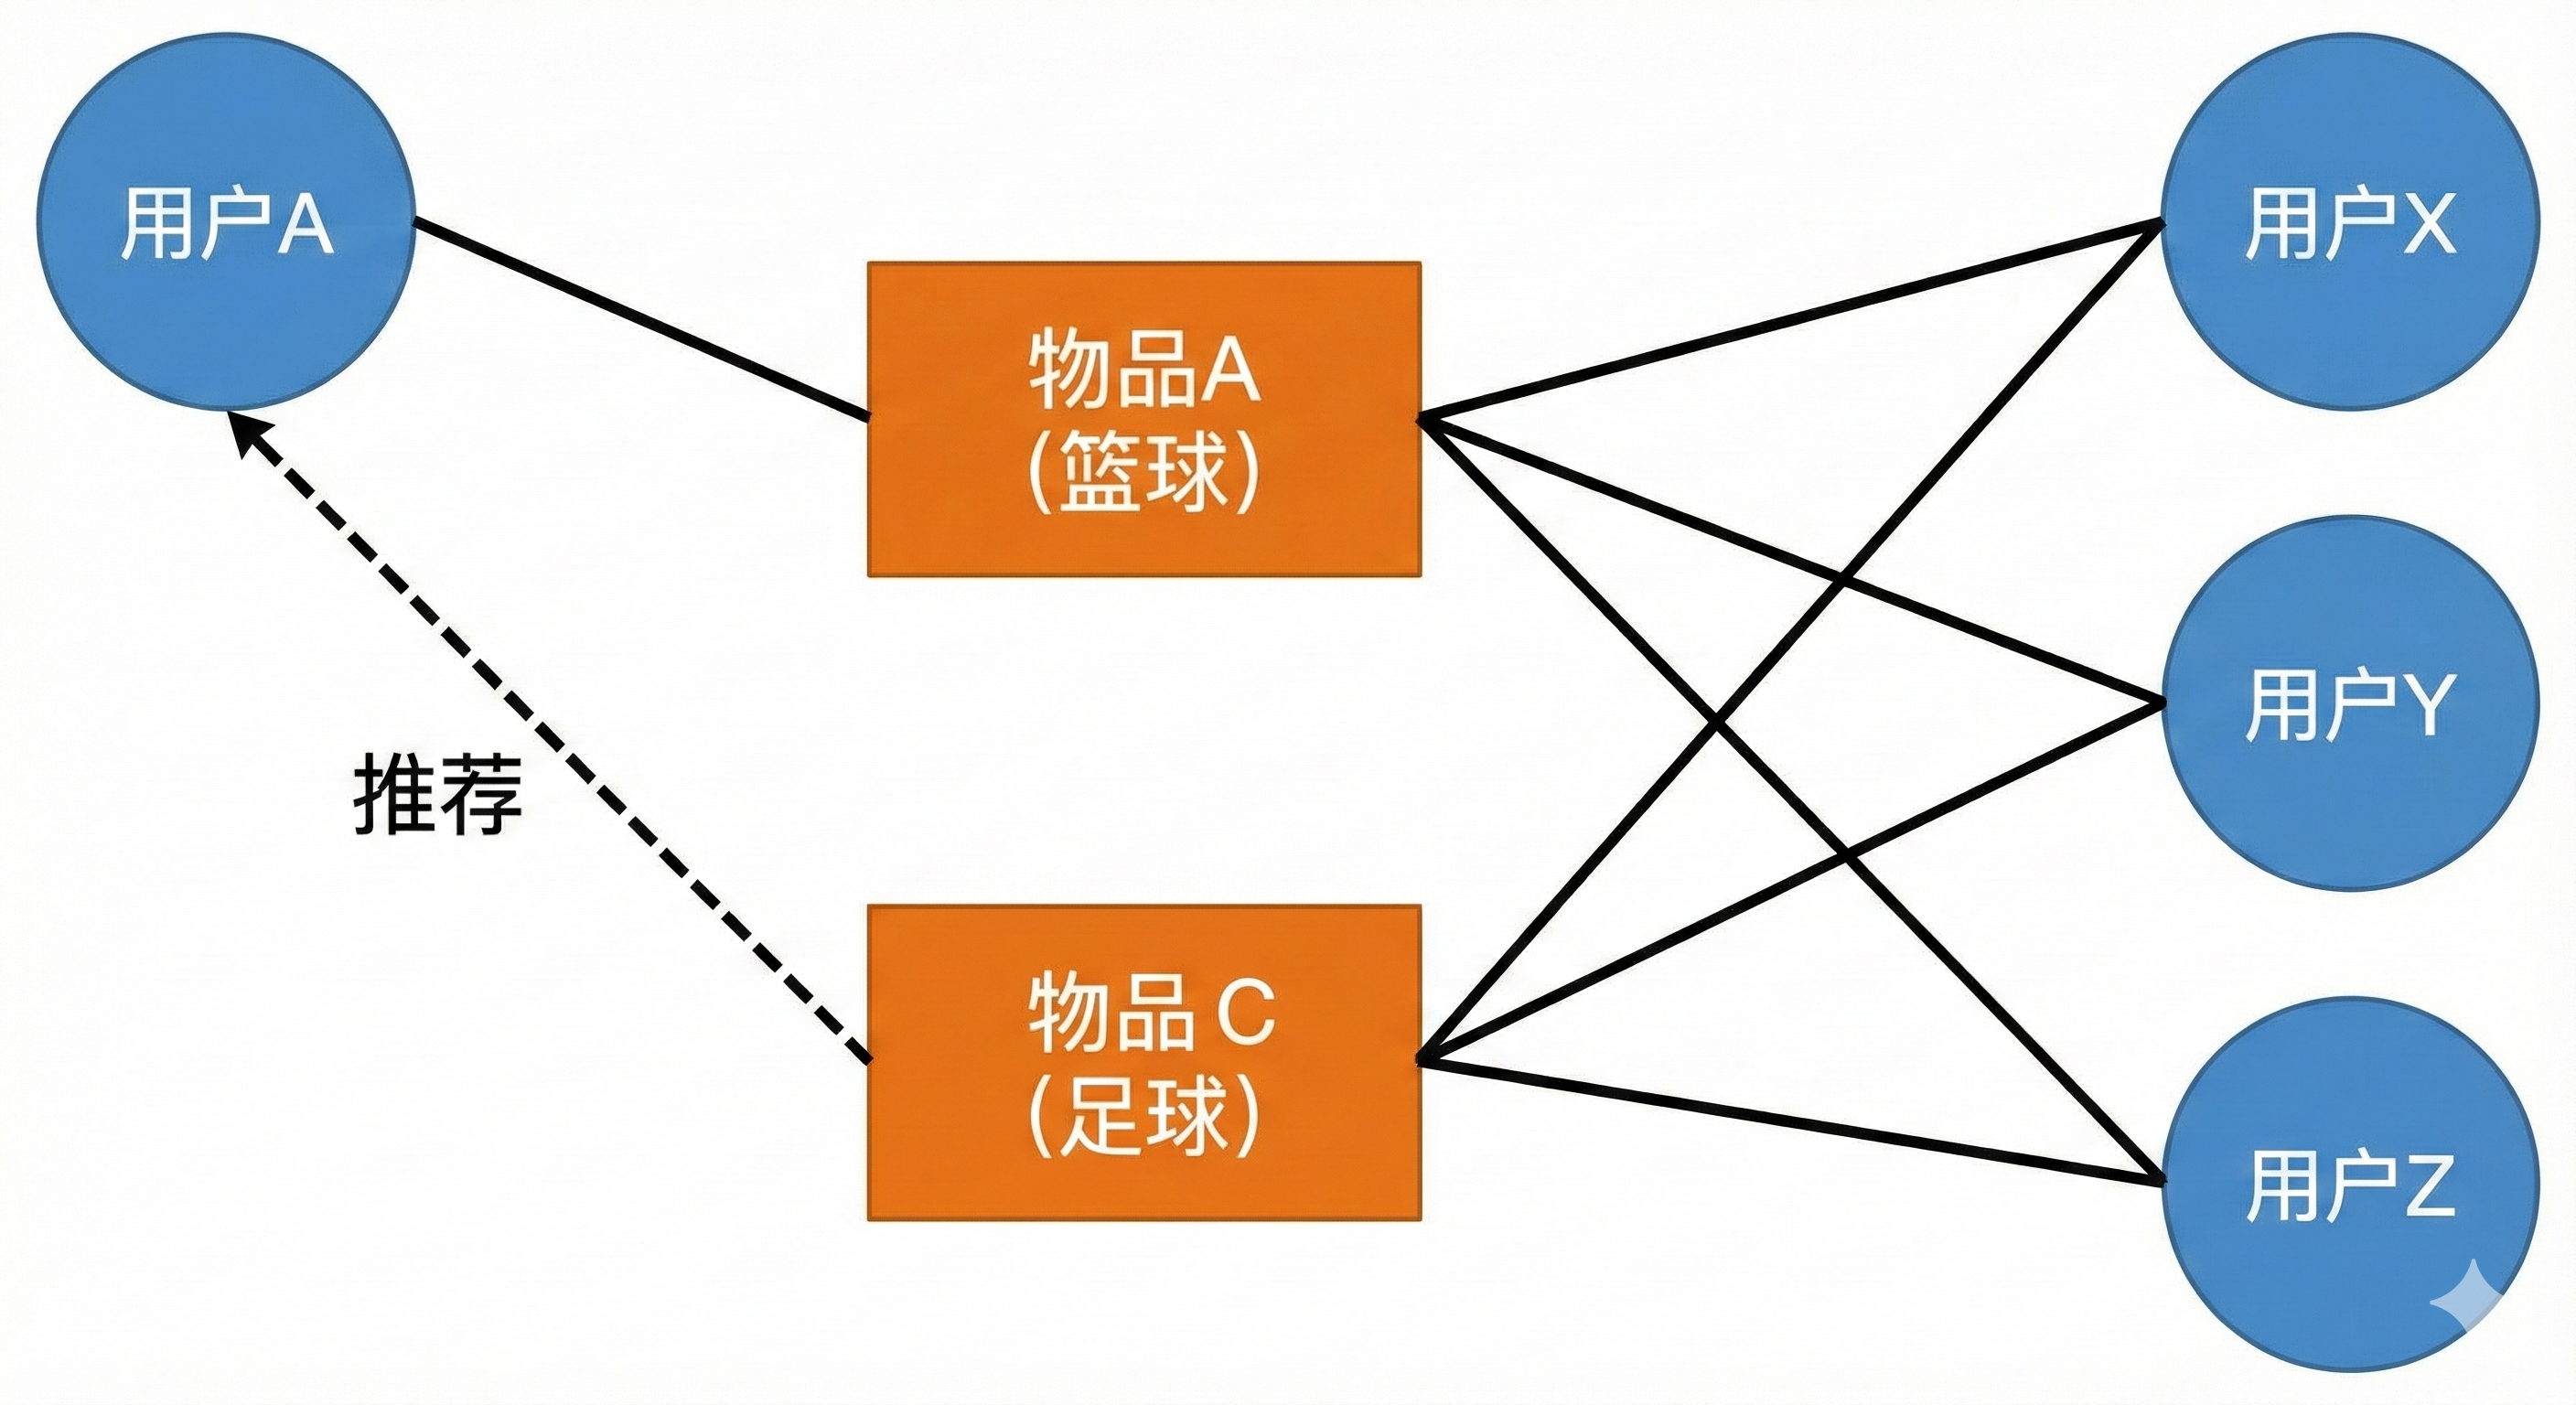
\includegraphics[width=0.75\textwidth]{images/CF.png}
    \caption{ItemCF 算法原理示意图}
    \label{fig:itemcf}
\end{figure}

    \textbf{优缺点分析:} 协同过滤算法具有模型通用性强、无需领域知识等优点。然而,其严重依赖历史交互数据,在面对\textbf{数据稀疏(Data Sparsity)}问题时推荐质量会明显下降;同时,对于无历史行为的新用户或新物品,存在严重的\textbf{冷启动(Cold Start)}问题\cite{qiao2018coldstart}。

    % --- (2) 矩阵分解 ---
    \item \textbf{矩阵分解方法(Matrix Factorization, MF)}
    
    矩阵分解是协同过滤算法在隐语义挖掘方向的延伸。其核心原理是将高维稀疏的用户-物品评分矩阵 $\mathbf{Y}$ 分解为两个低维的稠密矩阵:用户潜在特征矩阵 $\mathbf{P}$ 和物品潜在特征矩阵 $\mathbf{Q}$。通过将用户和物品映射到同一个低维隐向量空间,利用向量内积来预测用户对物品的评分或偏好程度。
    
    原理如图 \ref{fig:mf} 所示。

\begin{figure}[H]
    \centering
    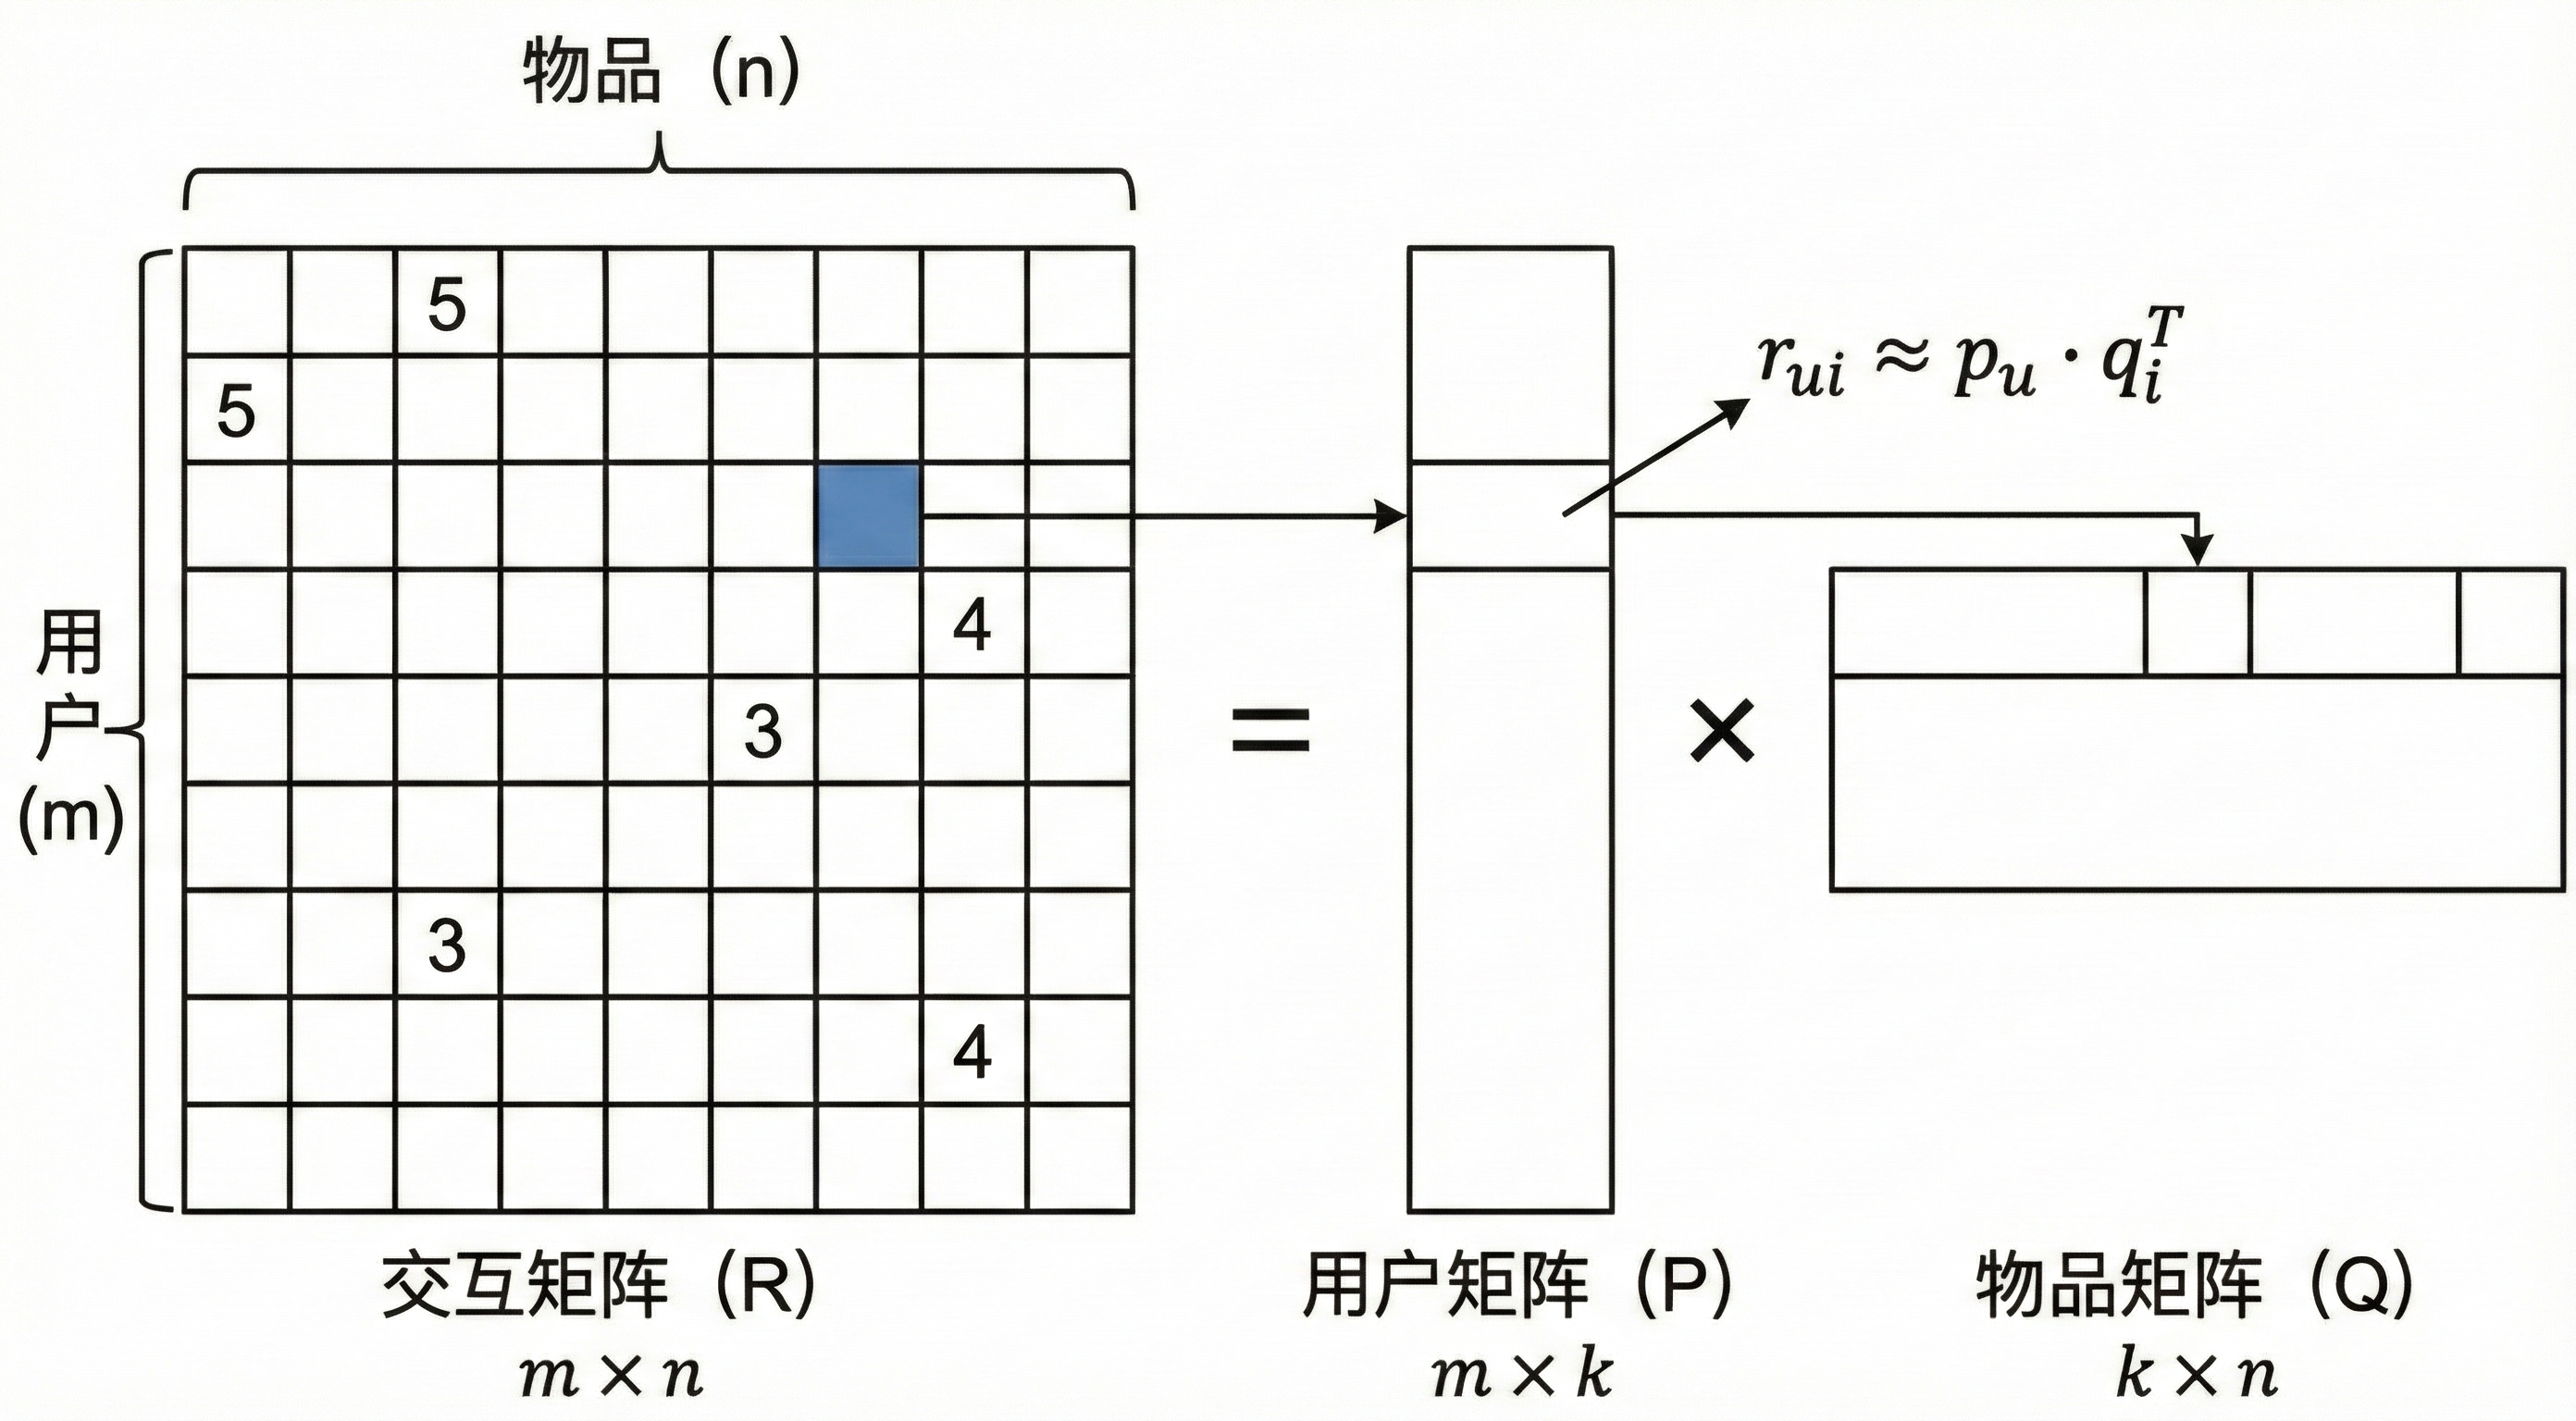
\includegraphics[width=0.8\textwidth]{images/matrix.png}
    \caption{矩阵分解(MF)示意图}
    \label{fig:mf}
\end{figure}

    % --- (3) 深度学习 ---
    \item \textbf{深度学习方法}
    
    深度学习技术的发展推动了神经网络在推荐系统中的应用。常见的方法包括:
    \begin{enumerate}
        \item \textbf{神经协同过滤(NCF):} 利用多层感知机(MLP)替代矩阵分解中的简单内积操作,以拟合用户与物品之间复杂的非线性交互函数。
        \item \textbf{序列推荐:} 利用循环神经网络(RNN)、Transformer 或 BERT 等模型建模用户行为的时间序列特征,捕捉用户兴趣的动态演化\cite{zhao2024multiinterest}。
    \end{enumerate}

    % --- (4) 基于图的推荐 ---
    \item \textbf{基于图的推荐系统}
    
    因为用户-物品交互数据天然具备图结构特性(即用户和物品可视为节点,交互行为视为边),基于图的推荐方法通过在图结构上来挖掘高阶协同信号。相较于传统方法,图方法能够利用多跳邻居信息,从而更准确地建模用户偏好\cite{he2020lightgcn, mao2021ultragcn}。关于该类方法的详细原理与演进,将在 \ref{sec:gnn_rec} 小节中进行详细阐述。
\end{enumerate}

\subsubsection{推荐系统常用的衡量指标}
为了全面、客观地评估推荐算法的性能,验证模型在 Top-K 推荐场景下的有效性,业界中常用的评估指标有:召回率(Recall)、归一化折损累计增益(NDCG)、曲线下面积(AUC)以及命中率(Hit Ratio)等。各指标的具体定义与计算公式如下:

\begin{enumerate}[label=(\arabic*)]
    \item \textbf{召回率(Recall@K)}
    
    Recall@K 是衡量推荐系统检索能力的核心指标,主要考察模型在 Top-K 推荐列表中覆盖用户真实感兴趣项目的比例。该指标关注的是“查全率”,即用户喜欢的物品有多少被模型成功找回。其数值越高,表明模型遗漏的正样本越少,推荐覆盖面越广。对于测试集中的用户集合 $\mathcal{U}$,其计算公式如式 \eqref{eq:recall} 所示:
    \begin{equation}
        \text{Recall}@K = \frac{1}{|\mathcal{U}|} \sum_{u \in \mathcal{U}} \frac{|\mathcal{R}_u \cap \mathcal{P}_u@K|}{|\mathcal{R}_u|}
        \label{eq:recall}
    \end{equation}
    式中,$\mathcal{R}_u$ 表示测试集中用户 $u$ 实际交互过的相关项目集合(Ground Truth);$\mathcal{P}_u@K$ 表示模型为用户 $u$ 生成的前 $K$ 个推荐项目列表;$|\cdot|$ 表示集合中元素的个数。

    \item \textbf{归一化折损累计增益(NDCG@K)}
    
    NDCG(Normalized Discounted Cumulative Gain)是评估推荐列表排序质量的重要指标。与 Recall 不同,NDCG 不仅关注模型是否推荐了正确的物品,还对物品在列表中的位置极其敏感。根据位置折损原则,排名越靠前的项目对最终分数的贡献越大。NDCG@K 的值介于 0 到 1 之间,值越高代表排序效果越符合用户偏好。其计算过程如式 \eqref{eq:ndcg} 所示:
    \begin{equation}
        \text{NDCG}@K = \frac{1}{|\mathcal{U}|} \sum_{u \in \mathcal{U}} \frac{\text{DCG}_u@K}{\text{IDCG}_u@K}
        \label{eq:ndcg}
    \end{equation}
    其中 $\text{DCG}_u@K$ 为折损累计增益,计算公式为 $\sum_{i=1}^{K} \frac{2^{rel_i} - 1}{\log_2(i+1)}$,$rel_i$ 表示第 $i$ 个位置的项目的相关性(在隐式反馈中,交互为1,否则为0);$\text{IDCG}_u@K$ 为理想状态下的最大累计增益,用于进行归一化处理。

    \item \textbf{曲线下面积(AUC)}
    
    AUC(Area Under the Curve)即 ROC 曲线下的面积,在推荐系统中常用于评估模型对正负样本的排序区分能力。从概率角度解释,AUC 代表了随机抽取一个正样本(用户喜欢的)和一个负样本(用户不喜欢的),模型对正样本的预测得分高于负样本得分的概率。AUC = 0.5 表示模型效果等同于随机猜测,AUC 越接近 1 表示模型的排序能力越强。其计算公式如式 \eqref{eq:auc} 所示:
    \begin{equation}
        \text{AUC} = \frac{1}{|\mathcal{U}|} \sum_{u \in \mathcal{U}} \frac{1}{|\mathcal{P}_u||\mathcal{N}_u|} \sum_{i \in \mathcal{P}_u} \sum_{j \in \mathcal{N}_u} \mathbb{I}(\hat{y}_{ui} > \hat{y}_{uj})
        \label{eq:auc}
    \end{equation}
    式中,$\mathcal{P}_u$ 和 $\mathcal{N}_u$ 分别表示用户 $u$ 的正样本集合和负样本集合;$\hat{y}_{ui}$ 和 $\hat{y}_{uj}$ 分别为模型对正样本 $i$ 和负样本 $j$ 的预测分数;$\mathbb{I}(\cdot)$ 为指示函数,当条件成立时取值为 1,否则为 0。

    \item \textbf{命中率(Hit@K)}
    
    Hit@K(Hit Ratio)是一种直观的准确性指标,用于衡量推荐列表 Top-K 中是否至少包含一个用户实际交互过的正样本。该指标通常用于留一法(Leave-One-Out)评估场景中。Hit@K 关注的是推荐结果的“存在性”,即模型是否“击中”了用户的兴趣点。其计算公式如式 \eqref{eq:hit} 所示:
    \begin{equation}
        \text{Hit}@K = \frac{1}{|\mathcal{U}|} \sum_{u \in \mathcal{U}} \mathbb{I}(|\mathcal{R}_u \cap \mathcal{P}_u@K| \geq 1)
        \label{eq:hit}
    \end{equation}
    式中,$\mathcal{R}_u$ 为用户 $u$ 的真实正样本集合,$\mathcal{P}_u@K$ 为模型推荐的前 $K$ 个项目。如果交集非空,说明推荐列表中包含至少一个正样本,指示函数记为 1,否则为 0。
\end{enumerate}

\subsection{图神经网络推荐技术}
\label{sec:gnn_rec}

\subsubsection{图神经网络(GNN)基本原理}
传统的协同过滤方法(如矩阵分解 MF)主要通过点积将用户和物品映射到同一潜在空间,这种方法本质上只建模了用户与物品的一阶线性关系,难以捕捉复杂的非线性结构信息。图神经网络(Graph Neural Networks, GNNs)通过在图结构上执行消息传递(Message Passing)机制,有效地解决了上述问题\cite{wu2021fedgnn, he2020lightgcn}。

GNN 的核心思想是利用图的拓扑结构,迭代地聚合邻居节点的特征信息,从而更新中心节点的表示。在推荐场景下,其基本原理主要包含以下三个步骤:

\textbf{(1)图结构定义与初始化}:定义用户集合 $\mathcal{U}$ 和物品集合 $\mathcal{V}$,交互图表示为 $\mathcal{G} = (\mathcal{U} \cup \mathcal{V}, \mathcal{E})$,其中 $\mathcal{E}$ 为边集。首先,为每个用户 $u$ 和物品 $v$ 初始化低维稠密向量(Embedding),记为 $\mathbf{e}_u^{(0)}$ 和 $\mathbf{e}_v^{(0)}$,作为第 0 层的输入特征。

\textbf{(2)消息传递与聚合}:消息传递是 GNN 的核心。在第 $l$ 层网络中,目标节点会收集其邻居节点的信息。对于用户节点 $u$,其聚合过程可以形式化为:
\begin{equation}
    \mathbf{m}_{\mathcal{N}_u}^{(l)} = \text{AGGREGATE}^{(l)} \left( \{ \mathbf{e}_i^{(l-1)} : i \in \mathcal{N}_u \} \right) 
    \label{eq:gnn_agg}
\end{equation}
其中,$\mathcal{N}_u$ 表示用户 $u$ 的邻居节点集合(即交互过的物品),$\mathbf{e}_i^{(l-1)}$ 是邻居节点在上一层的特征表示,$\text{AGGREGATE}(\cdot)$ 是聚合函数,常见的形式包括均值聚合(Mean Pooling)、最大值聚合(Max Pooling)或加权求和等。

\textbf{(3)特征更新与高阶协同}:在聚合了邻居信息后,模型结合节点自身的当前状态进行更新,生成新的节点表示:
\begin{equation}
    \mathbf{e}_u^{(l)} = \text{UPDATE}^{(l)} \left( \mathbf{e}_u^{(l-1)}, \mathbf{m}_{\mathcal{N}_u}^{(l)} \right)
    \label{eq:gnn_update}
\end{equation}
通过堆叠 $L$ 层 GNN 网络,节点 $u$ 的最终表示 $\mathbf{e}_u^{(L)}$ 实际上融合了其 $L$ 跳(L-hop)邻居的信息。这种机制使得模型能够显式地编码高阶协同信号(High-order Connectivity)。例如,通过“用户A-物品1-用户B-物品2”的路径,模型可以挖掘出具有相似偏好的潜在用户群体,缓解了数据稀疏性问题,提升了推荐的准确性\cite{wang2019kgat}。

\begin{figure}[H]
    \centering
    \includegraphics[width=0.9\textwidth]{images/图神经网络.png} 
    \caption{图神经网络算法原理示意图}
    \label{fig:gnn}
\end{figure}

\subsubsection{同构图和异构图}

\begin{enumerate}
    \item \textbf{同构图(Homogeneous Graph)}:
    
    同构图是图结构中最简单的形式,图中所有的顶点都属于同一类型,并且所有的边也都属于同一类型。同构图示例如图 \ref{fig:homo_graph} 所示,图中的顶点具有相同的语义和属性集合,边也具有相同的语义和属性集合。
    
    用数学语言描述,设图 $G=(V, E)$,其中 $V$ 是顶点的集合,$E$ 是边的集合。对于任意的顶点 $u, v \in V$,它们具有相同的类型;对于任意的边 $(u, v) \in E$,这些边也具有相同的类型。
\end{enumerate}

\begin{figure}[H]
    \centering
    \includegraphics[width=0.6\textwidth]{images/同构图.png} 
    \caption{同构图示意图}
    \label{fig:homo_graph}
\end{figure}

\begin{enumerate}
    \item \textbf{异构图(Heterogeneous Graph)}:
    
    异构图是指图中存在多种类型的节点和边,每种类型可能代表不同的实体或关系。在异构图中,节点和边的不同属性赋予了图更丰富的语义信息\cite{yan2024fedhgnn}。
    
    形式化地,给定异构图 $\mathcal{G} = (\mathcal{V}, \mathcal{E}, \mathcal{A}, \mathcal{R})$,其中 $\mathcal{V}$ 是顶点集,$\mathcal{E}$ 是边集,$\mathcal{A}$ 是顶点类型集合,$\mathcal{R}$ 是边类型集合。异构图包含两个映射函数:
    \begin{enumerate}
        \item 顶点类型映射函数 $\phi: \mathcal{V} \rightarrow \mathcal{A}$,将顶点映射到一个顶点类型集合 $\mathcal{A}$ 中的某一类型;
        \item 边类型映射函数 $\psi: \mathcal{E} \rightarrow \mathcal{R}$,将边映射到一个边类型集合 $\mathcal{R}$ 中的某一类型。
    \end{enumerate}
    且满足 $|\mathcal{A}| > 1$ 或者 $|\mathcal{R}| > 1$(即至少存在两种顶点类型或者两种边类型)。
\end{enumerate}
现实世界的网络结构往往呈现出高度的复杂性,包含多种类型的实体及它们之间错综复杂的交互关系。相比于传统的单一视图建模,采用异构图能够完整保留数据的结构异质性(Structural Heterogeneity),从而更精准地捕捉实体间深层次的语义关联与依赖信息。

\subsubsection{基于元路径的推荐}
在异构信息网络(HIN)中,由于节点和边类型的多样性,直接应用传统的同构图算法难以捕捉复杂的语义信息,为了解决这个问题,Sun 等人提出了元路径(Meta-path)的概念。

对于给定网络模式 $T_G = (\mathcal{A}, \mathcal{R})$,元路径 $\mathcal{P}$ 是定义在网络模式上形如 $\mathcal{A}_1 \xrightarrow{\mathcal{R}_1} \mathcal{A}_2 \xrightarrow{\mathcal{R}_2} \dots \xrightarrow{\mathcal{R}_l} \mathcal{A}_{l+1}$ 的序列。其中,$\mathcal{A}_i \in \mathcal{A}$ 表示节点类型,$\mathcal{R}_i \in \mathcal{R}$ 表示连接节点类型 $\mathcal{A}_i$ 与 $\mathcal{A}_{i+1}$ 的关系。元路径定义了起始节点类型 $\mathcal{A}_1$ 与目标节点类型 $\mathcal{A}_{l+1}$ 之间的一种复合关系 $R = \mathcal{R}_1 \circ \mathcal{R}_2 \circ \dots \circ \mathcal{R}_l$。

对于给定的元路径 $\mathcal{P}$,用户节点 $u$ 的基于元路径的邻居集合 $\mathcal{N}_u^{\mathcal{P}}$ 包含了所有通过该路径与 $u$ 建立连接的节点。在推荐模型的特征学习阶段,模型通过以下聚合函数(Aggregation Function)生成用户在该特定语义下的嵌入表示(Embedding):
\begin{equation}
    \mathbf{h}_u^{\mathcal{P}} = \text{AGGREGATE}_{\mathcal{P}} \left( \left\{ \mathbf{h}_v \mid v \in \mathcal{N}_u^{\mathcal{P}} \right\} \right)
\end{equation}
其中,$\mathbf{h}_v$ 表示邻居节点的初始特征向量,$\text{AGGREGATE}(\cdot)$ 通常采用平均池化(Mean Pooling)或注意力机制(Attention Mechanism)\cite{wang2019han}。例如,在“User-Movie-User”路径下,聚合操作实际上是在学习“与其观看历史相似的其他用户”的特征分布,从而捕捉协同过滤语义\cite{li2023metapath}。

\begin{figure}[H]
    \centering
    \includegraphics[width=0.75\textwidth]{images/元路径.png}
    \caption{异构图与元路径示意图}
    \label{fig:meta_path}
\end{figure}

\subsection{联邦学习概述}

联邦学习是由谷歌(Google)于 2016 年首次提出的一种新兴分布式机器学习范式,旨在打破"数据孤岛"并保护用户隐私\cite{li2025openfgl}。

其核心理念在于"\textbf{数据不动模型动}",即在不共享原始数据、保护数据隐私的同时,利用分布在不同客户端(Clients)的数据协同训练出一个全局模型。联邦学习通常采用\textbf{客户端-服务器(Client-Server)}架构\cite{deng2023survey}。

一轮标准的联邦学习训练包含以下四个步骤:

\begin{enumerate}
    \item \textbf{梯度发送(本地训练)} : 参与训练的客户端首先接收服务器下发的初始全局模型,利用本地数据进行训练,得到本地模型。训练完成后,客户端将计算出的加密梯度上传至服务器。

    \item \textbf{安全聚合} : 服务器收到各个参与客户端上传的加密梯度后,利用聚合算法(如安全聚合)对梯度进行汇总处理,从而更新全局模型。

    \item \textbf{模型返回} : 服务器将更新后的全局模型发送回所有参与训练的客户端。

    \item \textbf{模型更新} : 参与客户端收到最新的全局模型后,用其更新本地模型,准备进行下一轮训练。
\end{enumerate}

上述步骤不断迭代,直至模型收敛,最终获得可用的全局模型。

\begin{figure}[H]
    \centering
    \includegraphics[width=0.8\textwidth]{images/联邦推荐图.jpg} 
    \caption{联邦学习架构示意图}
    \label{fig:fl_overview}
\end{figure}

同时根据参与方数据的分布特性(即数据样本与特征空间的重叠情况),联邦学习通常被分为横向联邦学习、纵向联邦学习和联邦迁移学习三类\cite{guo2024fedgnn}。
\begin{enumerate}
    \item \textbf{横向联邦学习(Horizontal FL):} 主要适用于参与方数据特征空间重叠较多、但样本空间重叠较少的场景。这意味着不同参与方拥有相似的业务场景或数据结构,但服务于不同的用户群体。
    
    例如:不同的高校电子图书馆两者拥有相似的数据特征(均包含学生的论文下载记录、检索关键词、浏览时长等),但各自服务于不同的学生群体。通过横向联邦学习,双方可以联合利用更大规模的阅读行为数据,训练出泛化能力更强的论文推荐模型。
\end{enumerate}

\begin{figure}[H]
    \centering
    \includegraphics[width=0.8\textwidth]{images/横向联邦学习.png} 
    \caption{横向联邦学习示意图}
    \label{fig:horz_fl}
\end{figure}

\begin{enumerate}
    \item \textbf{纵向联邦学习(Vertical FL):} 主要适用于参与方数据样本空间重叠较多、但特征空间重叠较少的场景。这种情况常见于同一地区的不同机构之间,它们拥有同一批用户,但掌握该用户不同维度的属性数据。
    
    例如:一所高校的电子图书馆与该校的科研管理系统。两者服务于同一批师生用户(样本相同),但图书馆掌握用户的论文下载与阅读记录,而科研系统掌握用户的论文发表情况与课题申报信息。通过纵向联邦学习,可以将用户的"阅读输入"与"科研输出"数据相结合,构建画像更立体的推荐模型,向用户推荐更符合其科研产出方向的文献\cite{wang2025p4gcn}。
\end{enumerate}

\begin{figure}[H]
    \centering
    \includegraphics[width=0.8\textwidth]{images/纵向联邦学习.png} 
    \caption{纵向联邦学习示意图}
    \label{fig:vert_fl}
\end{figure}

\begin{enumerate}
    \item \textbf{迁移联邦学习(Transfer FL):} 主要适用于参与方数据样本空间与特征空间均存在较大差异,且少量重叠的场景,解决单边数据稀缺或标签不足的问题。 
    
    例如:英文计算机科学(CS)论文数据库与新兴的中文生物医学论文平台。两者的用户群体和数据特征均存在巨大差异。通过联邦迁移学习,可以在两者仅有的交叉学科(如生物信息学)重叠数据上进行对齐,将CS数据库中成熟的引文图谱结构知识迁移到生物医学平台,解决新兴平台因数据稀缺导致的推荐冷启动问题\cite{li2025fedcsr, chen2024fedgcdr}。
\end{enumerate}

\begin{figure}[H]
    \centering
    \includegraphics[width=0.8\textwidth]{images/迁移学习.png} 
    \caption{联邦迁移学习示意图}
    \label{fig:trans_fl}
\end{figure}

\subsection{对比学习}
对比学习(Contrastive Learning)是一种自监督学习方法,其核心思想是通过构造正负样本对,让模型学会区分相似与不相似的样本,从而获得具有判别性的表征\cite{crad2024multiview}。在推荐系统面临数据稀疏(Data Sparsity)和冷启动(Cold Start)问题时,对比学习能够利用数据自身的结构信息或增强视图构建辅助监督信号,从而在缺乏人工标注或交互记录的情况下,依然能学习出高质量的特征表示\cite{zhang2024ifedrec}。

对比学习的基本流程如下:对于一个输入样本 $x$(在推荐场景中可以是用户、物品或交互子图),通过两种不同的数据增强策略 $\mathcal{T}_1$ 和 $\mathcal{T}_2$ 分别生成两个增强视图 $\tilde{x}_i = \mathcal{T}_1(x)$ 和 $\tilde{x}_j = \mathcal{T}_2(x)$,它们被视为一对正样本(Positive Pair);同时,从同一个批次(Batch)的其他样本增强视图中采样,构建与当前视图语义相反的“负样本对”(Negative Pair)\cite{yu2022simgcl}。所有视图经过同一个编码器 $f(\cdot)$(如 GNN 或 Transformer)映射到特征空间,再经过投影头得到表示向量 $z_i = g(f(\tilde{x}_i))$ 和 $z_j = g(f(\tilde{x}_j))$。优化的目标是拉近正样本对在特征空间中的距离,同时推远负样本对的距离。在此过程中,最常用的损失函数是归一化温度缩放的对比损失(Normalized Temperature-scaled Cross Entropy Loss, NT-Xent),该损失在 SimCLR 等主流框架中被广泛采用\cite{wu2021sgl}。具体地,对于一对正样本 $(z_i, z_j)$,其损失函数定义为:
\begin{equation}
    \ell_{i,j} = - \log \frac{\exp(\text{sim}(z_i, z_j) / \tau)}{\sum_{k=1, k \neq i}^{2N} \mathbb{I}_{[k \neq i]} \exp(\text{sim}(z_i, z_k) / \tau)} 
    \label{eq:contrastive_loss}
\end{equation}
其中,$\text{sim}(u, v) = \frac{u^T v}{\|u\| \|v\|}$ 表示余弦相似度(Cosine Similarity);$\tau$ 是温度参数(Temperature Parameter),用于调节模型对困难负样本的关注程度及分布的平滑度;$N$ 是批次大小,分母中包含了除了自身以外的所有正负样本的相似度总和。整个批次的最终损失是所有正样本对损失的平均值,即:
\begin{equation}
    \mathcal{L} = \frac{1}{2N} \sum_{k=1}^{N} [\ell_{2k-1, 2k} + \ell_{2k, 2k-1}] 
    \label{eq:total_loss}
\end{equation}
这种方法不依赖于显式的用户行为标签,而是挖掘样本内在的结构一致性,能在缓解长尾分布和冷启动推荐中表现优异\cite{wang2025fedpcl}。

\begin{figure}[H]
    \centering
    \includegraphics[width=0.8\textwidth]{images/对比学习.png} 
    \caption{对比学习示意图}
    \label{fig:contrastive_learning}
\end{figure}

\subsection{模型剪枝与量化}
\label{sec:pruning_and_quantization}

\subsubsection{模型剪枝 (Model Pruning)}
模型剪枝是用于去除深度神经网络中的冗余参数与结构(Structure),以降低计算开销并加速推理过程的一种手段\cite{jiang2022fedmp}。 根据剪枝粒度的不同,主要分为以下两类:

\begin{enumerate}[label=(\arabic*)]
    \item \textbf{非结构化剪枝 (Unstructured Pruning)}:
    非结构化剪枝是一种细粒度(Fine-grained)的模型压缩方法。不同于结构化剪枝移除完整的通道或层,非结构化剪枝直接作用于神经网络的单个权重参数(Weight Level)。其核心思想是不受限于特定的网络拓扑结构,直接筛选并剔除(置零)那些对模型精度贡献较低的参数。

    \item \textbf{结构化剪枝 (Structured Pruning)}:
    该方法以卷积核、通道或完整的网络层为单位进行剪除。例如,基于权重的 $L_1$ 范数删除贡献较小的卷积通道。相比非结构化剪枝,结构化剪枝能直接改变网络拓扑,减少特征图维度,在通用硬件上即可显著降低显存占用并提升推理速度\cite{yi2023fedlpq}。
\end{enumerate}

\subsubsection{模型量化 (Model Quantization)}
模型量化是指将神经网络的权重参数(Weights)和激活值(Activations)从高精度表示(如 32 位浮点数 FP32)转换为低精度表示(如 8 位整数 INT8 或更低比特)的过程。 量化通过减少表示每个参数所需的比特数,能够显著降低模型的存储占用和内存带宽需求,并利用硬件的高效定点运算单元加速推理\cite{khan2025hufe}。根据量化实施阶段的不同,通常分为以下两类:

\begin{enumerate}[label=(\arabic*)]
    \item \textbf{训练后量化 (Post-Training Quantization, PTQ)}:
    PTQ 是在模型训练完成并收敛后进行的。它通常只需要少量的校准数据(Calibration Data)来计算量化参数(如缩放因子和零点),无需对整个模型进行重新训练。该方法实施简单、计算成本低,但在极低比特(如 4-bit 以下)情况下可能会导致较大的精度下降\cite{zeng2025feddt}。

    \item \textbf{量化感知训练 (Quantization-Aware Training, QAT)}:
    QAT 将量化操作引入到模型的训练或微调过程中。通过在训练的前向传播中模拟量化引入的误差(Quantization Noise),并利用直通估计器(Straight-Through Estimator, STE)在反向传播中更新梯度,使模型能够适应低精度表示。
\end{enumerate}
模型剪枝侧重于减少参数数量,而模型量化侧重于降低参数精度。在实际部署中,这两种技术通常是正交且互补的,常被组合使用(例如"先剪枝后量化")以在保证精度的同时最大化模型的压缩比\cite{openreview2024fedcomloc}。
\chapterblank
\newpage
\section{第三章\quad 基于属性-结构双视图对比学习的联邦异构图推荐算法}
\label{chap:fedascl}
\setcounter{section}{3} \setcounter{subsection}{0}

\subsection{问题说明}
\label{sec:motivation}
在联邦推荐系统的实际应用场景中,数据稀疏性与冷启动问题构成了限制模型性能的关键瓶颈。且随着联邦生态的扩展,冷启动的维度已从传统的“新用户/新物品”层级演变为更为棘手的“新客户端”层级\cite{zhang2024ifedrec}。

传统的联邦推荐算法主要依赖用户-物品交互图进行特征提取。然而,在新用户、新物品或新客户端接入初期,由于缺乏充分的历史交互记录,基于元路径的图卷积网络(GCN)往往难以捕捉有效的节点结构表征,导致推荐性能明显下降。与此相对的是,用户属性(如年龄、职业)和物品属性(如类别、描述文本)通常包含丰富的语义信息,且在冷启动阶段即可在客户端本地获取。若能利用这些属性信息,将为缓解交互稀疏性提供重要补充\cite{he2024hgca}。

此外,联邦学习固有的数据非独立同分布特性极易导致不同客户端之间出现模型参数的语义漂移,加剧了冷启动场景下的推荐偏差\cite{tan2023fedstar}。

为解决上述挑战,本章提出一种\textbf{基于属性-结构双视图对比学习的联邦异构图推荐算法(Federated Attribute-Structure Contrastive Learning, FedASCL)}。本章提出的算法通过双视图对比学习机制,将丰富的属性语义信息迁移至交互空间,并引入基于原型的语义对齐策略以矫正Non-IID带来的分布偏差,在保护隐私的同时完成冷启动场景下的高质量推荐\cite{wang2025fedpcl}。

\subsection{算法总体框架} 
\label{sec:framework}
FedASCL 采用常见的服务器-客户端联邦训练方式,其端到端执行流程包含以下六个步骤:

\textbf{(1)客户端本地双视图构建}:客户端首先基于用户和物品的原始属性构建\textbf{属性语义图},同时利用本地交互历史构建\textbf{交互结构图},形成互补的双视图输入。

\textbf{(2)双视图特征编码}:利用异构图神经网络分别对结构视图和属性视图进行编码,学习节点在不同视角下的高维特征表示。

\textbf{(3)细粒度跨视图对比}:在客户端本地执行跨视图对比学习,用于最大化属性语义表示与交互结构表示之间的互信息,完成语义迁移与增强\cite{crad2024multiview}。

\textbf{(4)原型语义对齐}:服务器聚合生成全局语义原型并下发,客户端利用这些原型对本地节点表示进行正则化约束,以缓解Non-IID导致的模型偏差\cite{zhang2024fedtgp}。

\textbf{(5)模型聚合与更新}:服务器收集各客户端上传的模型参数(或梯度),采用加权平均策略聚合后更新全局模型。

\textbf{(6)联合优化与推荐}:客户端利用预定义的元路径挖掘异构图中的高阶语义关联,结合推荐主任务损失与对比学习辅助损失进行联合反向传播,完成模型参数的闭环更新。

图~\ref{fig:fedascl_framework} 展示了FedASCL算法的总体架构,详细描述了各模块间的交互。

\begin{figure}[H]
    \centering
    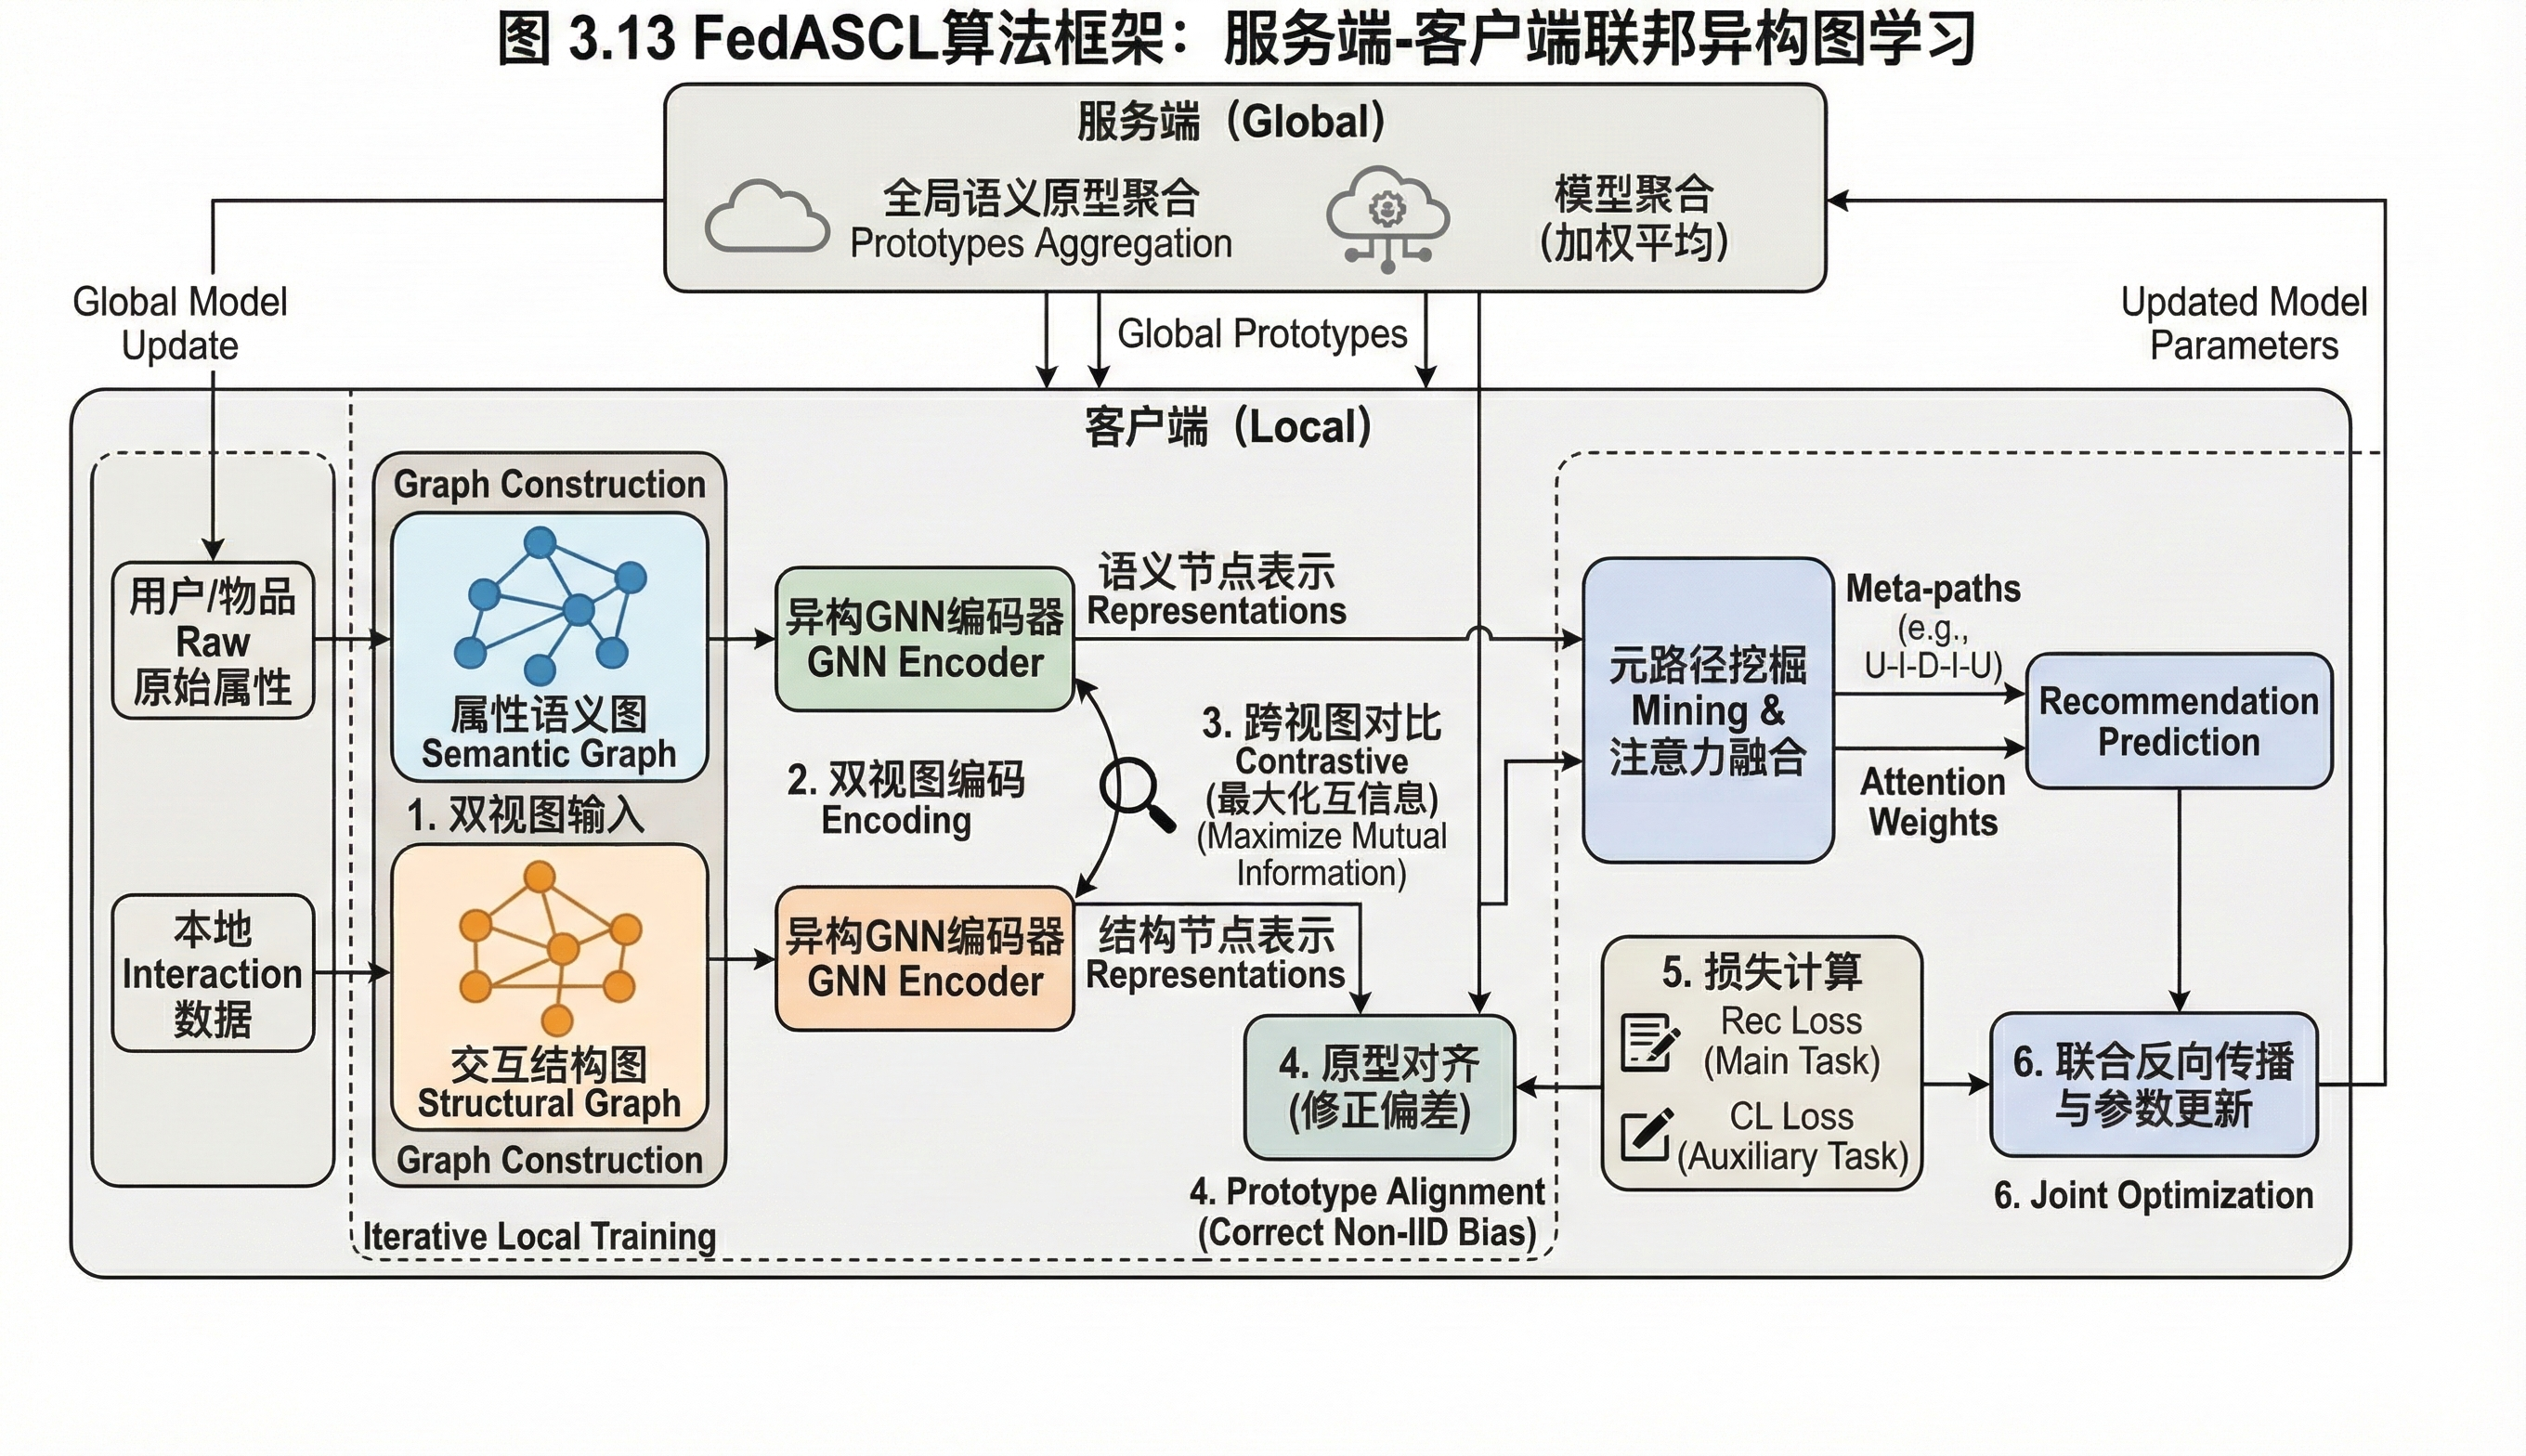
\includegraphics[width=0.95\textwidth]{images/model.png} 
    \caption{FedASCL算法总体架构示意图}
    \label{fig:fedascl_framework}
\end{figure}


\label{sec:core_modules}

\subsection{属性语义图构建}
\label{subsec:attr_sem_graph}

为弥补冷启动场景下交互结构的缺失,本章利用 $k$-近邻算法基于原始属性特征构建属性语义超图。该过程用于挖掘节点间潜在的语义关联,构建出显式的图结构供图神经网络学习\cite{he2024hgca}。具体构建流程形式化描述如下:

\subsubsection{特征预处理与向量化}
设联邦系统中的用户集合为 $\mathcal{U} = \{u_1, u_2, \dots, u_N\}$,物品集合为 $\mathcal{I} = \{i_1, i_2, \dots, i_M\}$。对于任意节点 $v \in \mathcal{U} \cup \mathcal{I}$,其原始属性集合包含离散型特征(如性别、类别)和连续型特征(如年龄、价格)。

为了将异构属性映射到统一的特征空间,首先对离散特征采用独热(One-hot)编码,对连续特征采用 Min-Max 归一化处理。假设节点 $v$ 处理后的特征向量为 $\mathbf{x}_v \in \mathbb{R}^{d_{attr}}$,其计算过程表示为:
\begin{equation}
    \mathbf{x}_v = \text{Concat}\left( \text{OneHot}(\mathbf{f}_{cat}), \frac{\mathbf{f}_{cont} - \min(\mathbf{f}_{cont})}{\max(\mathbf{f}_{cont}) - \min(\mathbf{f}_{cont})} \right)
\end{equation}
其中,$\mathbf{f}_{cat}$ 和 $\mathbf{f}_{cont}$ 分别表示原始的类别特征和连续特征向量,$\text{Concat}(\cdot)$ 为向量拼接操作。

\subsubsection{属性语义相似度计算}
在获得标准化的属性特征向量后,为了衡量节点间在语义层面的相似程度,本章采用余弦相似度作为度量标准。对于任意两个节点 $v_i$ 和 $v_j$,其语义相似度 $S_{ij}$ 定义为:
\begin{equation}
    S_{ij} = \cos(\mathbf{x}_i, \mathbf{x}_j) = \frac{\mathbf{x}_i^\top \mathbf{x}_j}{\|\mathbf{x}_i\|_2 \cdot \|\mathbf{x}_j\|_2}
\end{equation}
需要注意的是,在联邦学习场景下,为了保护隐私,上述计算通常限制在同类型节点之间(即用户-用户、物品-物品),或者在客户端本地利用部分脱敏的公共属性进行计算。

\subsubsection{kNN语义超图构建}
基于计算得到的相似度矩阵 $\mathbf{S}$,我们利用 $k$-近邻算法构建超图结构。超图 $\mathcal{G} = (\mathcal{V}, \mathcal{E})$ 由节点集合 $\mathcal{V}$ 和超边集合 $\mathcal{E}$ 组成,其中每条超边 $e \in \mathcal{E}$ 可以连接任意数量的节点,能够捕捉高阶语义关联。

对于每个节点 $v_i$,我们选取与其相似度最高的 $k$ 个节点构成邻居集合 $\mathcal{N}_k(v_i)$:
\begin{equation}
    \mathcal{N}_k(v_i) = \{ v_j \mid S_{ij} \in \text{Top-}k(S_{i \cdot}) \}
\end{equation}

为了构建超图,本章采用"节点即超边"的策略,即每个节点 $v_i$ 生成一条以自身为中心的超边 $e_i$,该超边包含节点 $v_i$ 及其所有 $k$ 个近邻。超图的结构通过关联矩阵 $\mathbf{H} \in \mathbb{R}^{|\mathcal{V}| \times |\mathcal{E}|}$ 来进行数学表达,其中 $|\mathcal{E}| = |\mathcal{V}|$。关联矩阵中的元素 $H_{ve}$ 定义如下:
\begin{equation}
    H_{ve} = \begin{cases} 
    1, & \text{if } v \in e \\
    0, & \text{otherwise}
    \end{cases}
\end{equation}
如果节点 $v_j$ 属于节点 $v_i$ 的 $k$ 近邻集合(即 $v_j \in \mathcal{N}_k(v_i) \cup \{v_i\}$),则在关联矩阵中 $H_{j, e_i} = 1$。

通过上述方式构建的属性语义超图关联矩阵 $\mathbf{H}$,将作为后续属性视图图神经网络的输入,用于聚合高阶语义特征。相较于普通图邻接矩阵,$\mathbf{H}$ 能够更灵活地建模"具有相似属性的一组节点"之间的群组关系,从而在冷启动阶段提供鲁棒的特征表示。

\begin{figure}[H]
    \centering
    \includegraphics[width=0.85\textwidth]{images/属性语义图构建.jpg} 
    \caption{属性语义图构建流程示意图}
    \label{fig:attr_sem_graph}
\end{figure}

\subsection{跨视图对比学习机制}
\label{subsec:cross_view_cl}
为实现从属性域到交互域的知识迁移,本章设计了细粒度的跨视图对比学习机制。其核心思想是基于互信息最大化原则,强制同一节点在“属性视图”和“结构视图”下的表示在共享的嵌入空间中保持语义一致性\cite{wang2025fedpcl}。实现过程包括双视图编码与对比优化两个阶段。

\subsubsection{双视图特征编码}
设 $\mathcal{V}$ 为节点集合(包含用户与物品)。为了捕获不同视角的语义,我们采用两个独立的异构图神经网络(HGNN)作为编码器。

\textbf{(1)结构视图编码}:基于用户-物品交互图 $\mathcal{G}_{stru}$,利用异构图卷积层聚合邻居信息。设 $\mathbf{h}_i^{(l)}$ 为节点 $i$ 在第 $l$ 层的隐藏状态,其更新规则为:
\begin{equation}
    \mathbf{z}_i^{stru} = \text{HGNN}_{stru}(\mathcal{G}_{stru}, \mathbf{X})
\end{equation}
其中 $\mathbf{z}_i^{stru}$ 是节点 $i$ 经过多层聚合后的结构及其上下文特征表示,$\mathbf{X}$ 为初始特征矩阵。结构视图侧重于捕获"协同过滤"信号。

\textbf{(2)属性视图编码}:基于 \ref{subsec:attr_sem_graph} 节构建的属性语义超图 $\mathcal{G}_{attr}$(对应关联矩阵 $\mathbf{H}$),采用超图卷积网络进行编码:
\begin{equation}
    \mathbf{z}_i^{attr} = \text{HGNN}_{attr}(\mathbf{H}, \mathbf{X}) = \sigma(\mathbf{D}_v^{-1/2} \mathbf{H} \mathbf{W}_e \mathbf{D}_e^{-1} \mathbf{H}^\top \mathbf{D}_v^{-1/2} \mathbf{X} \mathbf{\Theta})
\end{equation}
其中 $\mathbf{z}_i^{attr}$ 是节点 $i$ 的属性语义表示。该视图侧重于捕获"内容相似性"信号,对于冷启动节点而言,该向量是主要的推断依据。



\subsubsection{InfoNCE 损失函数推导}
为了对齐 $\mathbf{z}_i^{stru}$ 和 $\mathbf{z}_i^{attr}$,我们将同一节点在两个视图下的嵌入视为\textbf{正样本对},将该节点与其他节点在任意视图下的嵌入视为\textbf{负样本对}。

首先,定义两个向量 $\mathbf{u}, \mathbf{v}$ 之间的相似度度量函数 $\text{sim}(\cdot, \cdot)$,本文采用余弦相似度:
\begin{equation}
    \text{sim}(\mathbf{u}, \mathbf{v}) = \frac{\mathbf{u}^\top \mathbf{v}}{\|\mathbf{u}\| \cdot \|\mathbf{v}\|}
\end{equation}

我们采用 InfoNCE 损失函数来最大化正样本对之间的互信息下界。对于一个包含 $N$ 个节点的训练批次,节点 $i$ 的跨视图对比损失 $\mathcal{L}_{cl}^{(i)}$ 定义为:

\begin{equation}
    \mathcal{L}_{cl}^{(i)} = - \log \frac{\exp(\text{sim}(\mathbf{z}_i^{stru}, \mathbf{z}_i^{attr}) / \tau)}{\sum_{j=1, j \neq i}^{N} \underbrace{\exp(\text{sim}(\mathbf{z}_i^{stru}, \mathbf{z}_j^{attr}) / \tau)}_{\text{Inter-view Negatives}} + \sum_{j=1, j \neq i}^{N} \underbrace{\exp(\text{sim}(\mathbf{z}_i^{stru}, \mathbf{z}_j^{stru}) / \tau)}_{\text{Intra-view Negatives}}}
    \label{eq:cl_loss}
\end{equation}
为了简化计算,在实际部署中我们主要关注\textbf{跨视图负样本}(即分母的第一部分)。该损失函数通过拉近分子中的正样本对、推远分母中的负样本对,实现了特征空间的对齐\cite{wu2021sgl, yu2022simgcl}。

\subsubsection{温度系数 $\tau$ 的梯度传播分析}
公式中的 $\tau$ 是一个关键的超参数。虽然它仅是一个标量,但对梯度的传播机制和语义迁移效果有着决定性影响。

我们可以通过分析损失函数对负样本相似度 $s_{i,j} = \text{sim}(\mathbf{z}_i^{stru}, \mathbf{z}_j^{attr})$ 的梯度来理解 $\tau$ 的作用。根据链式法则,梯度 $\frac{\partial \mathcal{L}_{cl}}{\partial s_{i,j}}$ 为:
\begin{equation}
    \frac{\partial \mathcal{L}_{cl}}{\partial s_{i,j}} = \frac{1}{\tau} \cdot \frac{\exp(s_{i,j}/\tau)}{\sum_{k \neq i} \exp(s_{i,k}/\tau)} = \frac{1}{\tau} \cdot P_{i,j}
\end{equation}
其中 $P_{i,j}$ 可以理解为模型将负样本 $j$ 误判为正样本的相对概率(即负样本的"困难程度")。

\textbf{(1)当 $\tau \to 0$ (极小值)}:分布变得极度尖锐。此时,$P_{i,j}$ 仅在那些与锚点相似度极高($s_{i,j}$ 很大)的负样本上非零,而对容易区分的负样本几乎为0。这意味着模型将专注于挖掘\textbf{困难负样本},迫使属性视图学习到非常细粒度的区分特征。但也可能导致模型难以收敛或数值不稳定。

\textbf{(2)当 $\tau \to \infty$ (极大值)}:分布趋于均匀。所有负样本的权重 $P_{i,j}$ 趋于相等,模型对所有负样本一视同仁。这会导致梯度对于样本的区分能力变弱,难以学习到高质量的语义表征。

因此,$\tau$ 在本质上控制了模型对困难负样本的关注程度。在联邦推荐的冷启动场景中,我们需要适中的 $\tau$(如实验中设为 0.2),既能利用属性区分相似物品,又避免因过度关注噪声数据而导致模型过拟合。

\begin{figure}[H]
    \centering
    \includegraphics[width=0.85\textwidth]{images/跨视图对比机制.jpg} 
    \caption{跨视图对比学习机制示意图}
    \label{fig:cross_view_cl}
\end{figure}

\subsection{基于原型的语义对齐策略}
\label{subsec:prototype_alignment}
在联邦推荐场景下,不同客户端的数据分布往往存在显著的异构性。例如,某些客户端可能仅包含"科幻类"电影的交互记录,而另一部分客户端则集中于"爱情类"电影。这种局部数据的偏斜会导致本地训练得到的节点表示在嵌入空间中发生\textbf{语义漂移},即同一类别的物品在不同客户端的嵌入表示大相径庭,严重阻碍了全局模型的收敛与泛化\cite{tan2022fedproto}。

为解决该问题,本章引入\textbf{全局语义原型}机制。原型被定义为嵌入空间中某类语义特征的聚类中心。通过在服务器端聚合全局原型并下发,客户端利用这些"全局锚点"对本地表示进行正则化约束,从而实现语义对齐\cite{zhang2024fedtgp}。

\subsubsection{本地原型计算与上传}
在每一轮联邦训练的本地更新阶段结束后,客户端 $m$ 基于当前的节点嵌入表示计算本地语义原型。假设系统中设定了 $K$ 个潜在的语义类别(例如对应 $K$ 个物品类别或通过聚类得到的 $K$ 个簇)。

对于第 $k$ 个语义类别,客户端 $m$ 计算属于该类别的所有节点嵌入的均值作为本地原型 $\mathbf{c}_{m,k}^{(t)}$:
\begin{equation}
    \mathbf{c}_{m,k}^{(t)} = \frac{1}{|\mathcal{S}_{m,k}|} \sum_{i \in \mathcal{S}_{m,k}} \mathbf{z}_i^{(t)}
\end{equation}
其中,$\mathcal{S}_{m,k}$ 表示客户端 $m$ 中属于第 $k$ 类语义的节点集合(例如交互过的某类物品集合),$\mathbf{z}_i^{(t)}$ 为节点 $i$ 在第 $t$ 轮的双视图融合嵌入。

为了保护隐私,客户端不直接上传原始嵌入 $\mathbf{z}_i$,而是仅上传聚合后的原型 $\mathbf{c}_{m,k}^{(t)}$。此外,为满足差分隐私要求,我们在上传前对原型添加拉普拉斯噪声或高斯噪声 $\xi$:
\begin{equation}
    \tilde{\mathbf{c}}_{m,k}^{(t)} = \mathbf{c}_{m,k}^{(t)} + \xi, \quad \xi \sim \text{Laplace}(0, \frac{\Delta}{\epsilon})
\end{equation}

\subsubsection{全局原型聚合}
服务器收到各参与客户端上传的带噪本地原型后,执行加权聚合操作,生成全局语义原型 $\mathbf{C}^{(t)} = \{ \mathbf{c}_1^{(t)}, \dots, \mathbf{c}_K^{(t)} \}$。

第 $k$ 个全局原型的计算公式为:
\begin{equation}
    \mathbf{c}_k^{(t)} = \frac{\sum_{m \in \mathcal{M}^{(t)}} |\mathcal{S}_{m,k}| \cdot \tilde{\mathbf{c}}_{m,k}^{(t)}}{\sum_{m \in \mathcal{M}^{(t)}} |\mathcal{S}_{m,k}|}
\end{equation}
其中 $\mathcal{M}^{(t)}$ 是当前轮次参与训练的客户端集合。全局原型代表了该类语义在所有客户端视角下的“平均”或“公允”表示,随后被广播回所有客户端。

\subsubsection{本地语义对齐损失}
客户端接收到全局原型 $\mathbf{C}^{(t)}$ 后,将其作为正则化约束引入本地训练。我们的目标是:让本地节点的嵌入 $\mathbf{z}_i$ 尽可能靠近其所属类别的全局原型 $\mathbf{c}_{type(i)}$,同时远离其他类别的原型 $\mathbf{c}_{j} (j \neq type(i))$。

因此,我们设计了基于原型的对比对齐损失(Prototype-based Contrastive Loss):
\begin{equation}
    \mathcal{L}_{proto} = \sum_{i \in \mathcal{B}} - \log \frac{\exp(\mathbf{z}_i \cdot \mathbf{c}_{type(i)}^{(t)} / \tau_p)}{\sum_{k=1}^K \exp(\mathbf{z}_i \cdot \mathbf{c}_k^{(t)} / \tau_p)}
    \label{eq:proto_loss}
\end{equation}
其中,$\mathcal{B}$ 为本地训练批次,$type(i)$ 指示节点 $i$ 所属的语义类别,$\tau_p$ 为原型对比的温度系数。

该策略的作用主要体现在以下两个方面:

\textbf{(1)纠偏作用}:即使本地数据分布极度倾斜(例如全是动作片),全局原型也能告诉本地模型"爱情片"大概在嵌入空间的哪个位置,从而防止本地模型为了拟合局部数据而破坏了整体语义空间的结构。

\textbf{(2)冷启动增强}:对于新接入的冷启动客户端,由于缺乏交互,其初始嵌入往往是随机或基于属性粗糙生成的。全局原型为其提供了一个高质量的初始化参考系,使其能快速对齐到全局分布。

\begin{figure}[H]
    \centering
    \includegraphics[width=0.85\textwidth]{images/基于原型的语义对齐策略.jpg} 
    \caption{基于原型的语义对齐策略示意图}
    \label{fig:prototype_alignment}
\end{figure}

\subsection{基于元路径的推荐与联合优化}
\label{subsec:metapath_rec}

在通过双视图编码与对比学习获得高质量的节点表示后,FedASCL 算法利用元路径(Meta-path)机制来捕捉异构图中隐含的高阶语义关联,并执行最终的推荐任务。

\subsubsection{元路径定义与语义提取}
元路径 $\Phi$ 定义为连接网络模式中节点类型的复合关系序列,即 $A_1 \xrightarrow{R_1} A_2 \xrightarrow{R_2} \dots \xrightarrow{R_l} A_{l+1}$。在推荐场景中,不同的元路径代表了不同的语义偏好。本章定义了以下两类核心元路径集合 $\mathcal{P} = \{\Phi_1, \Phi_2, \dots, \Phi_P\}$:

\textbf{(1)协同关联路径}:如"用户-物品-用户"(U-I-U),表示购买过相同物品的用户可能具有相似偏好;

\textbf{(2)属性关联路径}:如"用户-属性-用户"(U-A-U)或"物品-类别-物品"(I-C-I),利用属性图构建的语义连接,缓解交互稀疏带来的信息匮乏\cite{li2023metapath}。


对于特定的元路径 $\Phi_p$,我们采用路径特定的 GCN 聚合该路径下的邻居信息,得到节点 $i$ 在该路径下的语义特定嵌入 $\mathbf{z}_i^{\Phi_p}$。

\subsubsection{语义级注意力融合机制}
由于不同元路径对用户意图的贡献度不同(例如,对于冷启动用户,属性路径 U-A-U 的重要性可能高于协同路径 U-I-U),简单的平均融合无法适应复杂的联邦场景。因此,我们设计了语义级注意力机制(Semantic-level Attention)来自适应地学习各元路径的权重\cite{wang2019han}。

首先,将各元路径下的节点嵌入 $\mathbf{z}_i^{\Phi_p}$ 输入到一个非线性变换中,计算其重要性分数:
\begin{equation}
    w_{\Phi_p} = \frac{1}{|\mathcal{V}|} \sum_{i \in \mathcal{V}} \mathbf{q}^\top \cdot \tanh(\mathbf{W}_{att} \mathbf{z}_i^{\Phi_p} + \mathbf{b}_{att})
\end{equation}
其中,$\mathbf{W}_{att}$ 和 $\mathbf{b}_{att}$ 是可学习的权重矩阵和偏置向量,$\mathbf{q}$ 是语义级别的注意力向量。

随后,利用 Softmax 函数对重要性分数进行归一化,得到最终的元路径权重 $\beta_{\Phi_p}$:
\begin{equation}
    \beta_{\Phi_p} = \frac{\exp(w_{\Phi_p})}{\sum_{p'=1}^P \exp(w_{\Phi_{p'}})}
\end{equation}

最后,基于学习到的权重对不同元路径的嵌入进行加权求和,得到融合了多重语义的最终节点表示 $\mathbf{z}_i^*$:
\begin{equation}
    \mathbf{z}_i^* = \sum_{p=1}^P \beta_{\Phi_p} \cdot \mathbf{z}_i^{\Phi_p}
\end{equation}
该机制使得模型能够根据数据特性自动调整对结构信息与属性信息的依赖程度。

\subsubsection{评分预测与主任务损失}
基于融合后的用户最终表示 $\mathbf{z}_u^*$ 和物品最终表示 $\mathbf{z}_i^*$,我们采用内积操作预测用户 $u$ 对物品 $i$ 的偏好评分 $\hat{y}_{ui}$:
\begin{equation}
    \hat{y}_{ui} = (\mathbf{z}_u^*)^\top \mathbf{z}_i^*
\end{equation}

为了优化推荐排序性能,本章采用贝叶斯个性化排序损失作为主任务损失函数。BPR 假设观察到的交互(正样本)评分应高于未观察到的交互(负样本)。对于训练集中的三元组 $(u, i, j)$,其中 $i$ 为正样本物品,$j$ 为负样本物品,主任务损失定义为:
\begin{equation}
    \mathcal{L}_{rec} = \sum_{(u,i,j) \in \mathcal{D}} - \ln \sigma(\hat{y}_{ui} - \hat{y}_{uj}) + \lambda \|\Theta\|_2^2
\end{equation}
其中 $\sigma(\cdot)$ 是 Sigmoid 函数,$\Theta$ 表示模型参数,最后一项为 $L_2$ 正则化项。

\subsubsection{多任务联合优化}
为了在联邦训练中同时兼顾推荐准确性、冷启动适应性与 Non-IID 鲁棒性,我们将前文提出的跨视图对比损失 $\mathcal{L}_{cl}$(公式 \ref{eq:cl_loss})和原型对齐损失 $\mathcal{L}_{proto}$(公式 \ref{eq:proto_loss})作为辅助任务,构建最终的联合优化目标函数:
\begin{equation}
    \mathcal{L}_{total} = \mathcal{L}_{rec} + \lambda_1 \mathcal{L}_{cl} + \lambda_2 \mathcal{L}_{proto}
\end{equation}
其中,$\lambda_1$ 和 $\lambda_2$ 是用于平衡不同任务权重的超参数。在客户端本地训练过程中,通过反向传播算法最小化 $\mathcal{L}_{total}$ 来更新本地模型参数,随后上传至服务器进行聚合。

% 用mdframed包裹algorithm,添加黑色边框(需要安装 mdframed 包)
% 暂时注释掉 mdframed,使用普通边框
\subsection{算法流程}
\begin{algorithm}[H]  % H 表示强制在当前位置,不浮动
    \caption{FedASCL 联邦训练算法流程}
    \label{alg:fedasclrc}
    \begingroup
    \small
    \setlength{\baselineskip}{0.78\baselineskip}  % 收紧行距,使算法流程在一页内
    \setlength{\lineskip}{0.5pt}
    \begin{algorithmic}[1] % [1]表示每行编号
        \Require 用户集合 $\mathcal{U}$,物品集合 $\mathcal{I}$,属性特征 $\mathbf{X}$;\\
                交互图 $\mathcal{G}_{stru}$;\\
                联邦全局轮次 $T$,本地训练轮次 $E$,学习率 $\eta$;\\
                超参数:近邻数 $k$,温度系数 $\tau, \tau_p$,损失权重 $\lambda_1, \lambda_2$。
        \Ensure 训练好的全局模型参数 $\Theta^*$。

        % 服务器初始化
        \State \textbf{Server Initialization:} 初始化全局模型参数 $\Theta^{(0)}$ 和全局语义原型 $\mathbf{C}^{(0)}$。

        % 阶段一:联邦训练循环

        \For{$t = 1, 2, \dots, T$}
            \State 服务器随机选取活跃客户端集合 $\mathcal{M}^{(t)}$;
            \State 服务器下发全局参数 $\Theta^{(t-1)}$ 和全局原型 $\mathbf{C}^{(t-1)}$ 至客户端;
            
            % 客户端并行训练
            \For{each client $m \in \mathcal{M}^{(t)}$}
     
              
                \If{$t=1$} 
                    \State \textbf{视图构建 (\text{Sec 3.3}):} 基于公式 (\text{3.1})-(\text{3.4}),利用kNN构建属性语义超图 $\mathcal{G}_{attr}$(仅首次训练执行);
                \EndIf
                \State 加载全局参数 $\Theta_m \leftarrow \Theta^{(t-1)}$;
                
                % 本地训练轮次
                \For{$e = 1, \dots, E$}
                    \State \textbf{特征编码 (\text{Sec 3.4.1}):} 
                    \State \qquad 计算结构视图表示:$\mathbf{Z}^{stru} \leftarrow \text{HGNN}_{stru}(\mathcal{G}_{stru}, \mathbf{X})$;
                    \State \qquad 计算属性视图表示:$\mathbf{Z}^{attr} \leftarrow \text{HGNN}_{attr}(\mathcal{G}_{attr}, \mathbf{X})$;
                    
                    \State \textbf{损失计算 (\text{Sec 3.6.4}):}
                    \State \qquad 跨视图对比损失:$\mathcal{L}_{cl}$(\text{Eq. 3.8});
                    \State \qquad 原型对齐损失:$\mathcal{L}_{proto}$(\text{Eq. 3.13});
                    \State \qquad 推荐主任务损失:$\mathcal{L}_{rec}$(\text{Eq. 3.18});
                    \State \qquad 总损失:$\mathcal{L}_{total} = \mathcal{L}_{rec} + \lambda_1 \mathcal{L}_{cl} + \lambda_2 \mathcal{L}_{proto}$;
                    
                    \State \textbf{参数更新:} $\Theta_m \leftarrow \Theta_m - \eta \nabla \mathcal{L}_{total}$;
                \EndFor
                
                \State \textbf{原型计算 (\text{Sec 3.5.1}):} 计算本地原型 $\mathbf{c}_{m}^{(t)}$,并添加隐私噪声以满足差分隐私(\text{Eq. 3.10-3.11});
                \State 上传本地模型 $\Theta_m$ 和加噪后的本地原型 $\tilde{\mathbf{c}}_{m}^{(t)}$ 至服务器;
            \EndFor

            % 服务器端聚合
            \State \textbf{模型聚合:} $\Theta^{(t)} \leftarrow \sum_{m \in \mathcal{M}^{(t)}} \frac{|\mathcal{D}_m|}{|\mathcal{D}|} \Theta_m$(按客户端数据量加权平均);
            \State \textbf{原型聚合:} 基于加权平均更新全局语义原型 $\mathbf{C}^{(t)}$(\text{Eq. 3.12});
        \EndFor
        \State \Return 最终全局模型参数 $\Theta^{(T)}$(即 $\Theta^*$)。
    \end{algorithmic}
    \endgroup
\end{algorithm}
\subsection{复杂度分析}
\label{sec:complexity_analysis}

本节从时间复杂度和空间复杂度两个维度对 FedASCL 算法进行理论分析。在此,设系统中节点总数为 $N$(包括用户和物品),交互边总数为 $M$。设特征嵌入维度为 $d$,GCN/HGNN 的网络层数为 $L$,训练时的批次大小为 $B$。

\subsubsection{时间复杂度分析}
FedASCL 的时间开销主要由三个阶段组成:属性图构建、双视图特征编码与联合优化。

在预处理阶段,我们需要基于 $k$-近邻算法构建属性语义超图。

\textbf{(1)相似度计算与排序}:对于拥有 $N$ 个节点的集合,暴力计算两两余弦相似度并排序的时间复杂度为 $O(N^2 d + N^2 \log N)$。考虑到在联邦学习场景下,该步骤通常在客户端本地对局部数据子集 $n_m$ ($n_m \ll N$) 执行,或利用局部敏感哈希(LSH)等近似最近邻搜索技术加速,实际复杂度可降低至 $O(N \cdot k \cdot d)$。

\textbf{(2)超图关联矩阵生成}:选取 Top-$k$ 邻居构建关联矩阵 $\mathbf{H}$ 的操作是线性的,复杂度为 $O(N \cdot k)$。
需要注意的是,该过程通常作为一次性离线计算完成,不计入每轮训练的实时开销中。

在每一轮训练的前向传播中,时间开销主要来自图卷积操作:

\textbf{(1)结构视图 (Structure View)}:利用用户-物品二部图 $\mathcal{G}_{stru}$ 进行消息传递。由于 $\mathcal{G}_{stru}$ 是稀疏图,利用稀疏矩阵乘法优化,单层卷积的复杂度与边数呈线性关系,即 $O(M \cdot d)$。对于 $L$ 层网络,总开销为 $O(L \cdot M \cdot d)$。

\textbf{(2)属性视图 (Attribute View)}:基于超图关联矩阵 $\mathbf{H}$ 进行卷积。$\mathbf{H}$ 中每个节点连接 $k$ 个邻居,因此非零元素个数为 $N(k+1)$。超图卷积操作 $\mathbf{H}\mathbf{H}^\top \mathbf{X}$ 的复杂度主要取决于这些非零元素,约为 $O(L \cdot N \cdot k \cdot d)$。
由于 $k$ 通常较小(实验中设为 5-10),且 $M \gg N$,属性视图的引入并未明显增加图传播的数量级。

\textbf{(1)跨视图对比损失 ($\mathcal{L}_{cl}$)}:直接在全图上计算 InfoNCE 需要 $O(N^2 d)$ 的复杂度,这在计算上是不可接受的。本章采用基于批次(Batch-wise)的训练策略,仅在大小为 $B$ 的批次内计算正负样本对的相似度。此时复杂度降低为 $O(B^2 d)$。由于 $B \ll N$,该开销极低。

\textbf{(2)原型对齐损失 ($\mathcal{L}_{proto}$)}:计算节点与 $K$ 个全局原型的相似度,复杂度为 $O(B \cdot K \cdot d)$。其中 $K$ 为语义类别数(常数级)。

\textbf{(3)推荐主任务损失 ($\mathcal{L}_{rec}$)}:计算 BPR 损失仅涉及正负样本对的内积,复杂度为 $O(B \cdot d)$。

因此,FedASCL 单次迭代的总时间复杂度为:
\begin{equation}
    T_{total} \approx O\Big( L(M + Nk)d + B^2d + BKd \Big)
\end{equation}
由于 $M$ 通常远大于 $Nk$ 和 $B^2$,算法的主导复杂度仍为 $O(LMd)$,这与标准的 LightGCN 等基准模型保持一致\cite{he2020lightgcn}。这表明 FedASCL 在引入对比学习增强语义表示的同时,未引入过高的计算负担。

\subsubsection{空间复杂度分析}
空间复杂度主要涉及模型参数、图结构数据以及中间嵌入表示的存储。

\textbf{(1)图结构存储}:我们采用压缩稀疏行(CSR)格式存储邻接矩阵。
\begin{enumerate}[label=\arabic*.]
    \item 结构图 $\mathcal{G}_{stru}$ 需要存储 $2M$ 条有向边,空间复杂度为 $O(M)$。
    \item 属性超图 $\mathcal{G}_{attr}$ 的关联矩阵 $\mathbf{H}$ 包含 $N(k+1)$ 个非零项,空间复杂度为 $O(Nk)$。
\end{enumerate}

\textbf{(2)模型参数与嵌入}:
\begin{enumerate}[label=\arabic*.]
    \item \textbf{节点嵌入}:存储所有用户和物品的 $d$ 维嵌入向量,空间开销为 $O(N \cdot d)$。这是推荐系统内存占用的主要部分。
    \item \textbf{网络权重}:GCN 和 HGNN 的变换矩阵通常较小(如 $d \times d$),空间复杂度为 $O(L \cdot d^2)$。
    \item \textbf{全局原型}:存储 $K$ 个全局原型向量,开销为 $O(K \cdot d)$,相对于节点嵌入可忽略不计。
\end{enumerate}

综上,FedASCL 的总空间复杂度为 $O(M + Nk + Nd)$。该空间占用与节点数和边数呈线性关系,证明了模型在大规模稀疏数据集上的可扩展性。

\subsection{实验设置}
\label{subsec:exp_setup}

为验证 FedASCL 框架的有效性,本章在三个公开数据集上做实验,围绕以下三个问题展开:
\begin{enumerate}
    \item \textbf{RQ1 (总体性能)}:FedASCL 在常规联邦推荐场景下,是否优于现有的基线方法?
    \item \textbf{RQ2 (冷启动适应性)}:在缺乏交互历史的冷启动场景下,双视图机制能否提升推荐质量?
    \item \textbf{RQ3 (鲁棒性与消融)}:面对 Non-IID 数据分布,算法是否具有鲁棒性?各核心组件(对比学习、原型对齐)贡献如何?
\end{enumerate}

\subsubsection{数据集与预处理}
实验选取了三个具有丰富属性信息的代表性数据集:\textbf{MovieLens-1M}、\textbf{Yelp} 和 \textbf{ACM}。具体统计信息见表~\ref{tab:dataset_stat}。

\begin{table}[H]
    \centering
    \caption{实验数据集统计信息}
    \label{tab:dataset_stat}
    \renewcommand{\arraystretch}{1.2}
    \begin{tabular}{lcccc}
        \toprule
        \textbf{Dataset} & \textbf{\# Users} & \textbf{\# Items} & \textbf{\# Interactions} & \textbf{Sparsity} \\
        \midrule
        MovieLens-1M & 6,040 & 3,706 & 1,000,209 & 95.53\% \\
        Yelp & 15,480 & 12,095 & 635,403 & 99.66\% \\
        ACM & 25,678 & 18,432 & 845,120 & 99.82\% \\
        \bottomrule
    \end{tabular}
\end{table}

为了模拟联邦学习环境,我们利用狄利克雷分布 $\text{Dir}(\alpha)$ 将交互数据划分到 $N_{client}=50$ 个客户端中。其中 $\alpha$ 控制数据异构程度,$\alpha$ 越小表示 Non-IID 程度越高。除非特殊说明,默认设置 $\alpha=1.0$。

\subsubsection{对比基线模型}
本实验选取了三类主流算法作为对比基准:经典联邦推荐 FedNCF\cite{luo2024perfedrec},联邦图神经网络 FedGNN\cite{wu2021fedgnn}、FedPerGNN\cite{wu2022fedpergnn}、FedHGNN\cite{yan2024fedhgnn},以及联邦原型学习 FedProto\cite{tan2022fedproto}。

\subsubsection{参数设置}
评估指标采用 HR@K 和 NDCG@K($K=10, 20$;分别表示前 $K$ 个推荐结果中的命中率与前 $K$ 位的归一化折损累积增益)。关键超参数设置如下:属性近邻数 $k=10$,对比学习温度 $\tau=0.2$,原型温度 $\tau_p=0.5$,损失权重 $\lambda_1=\lambda_2=0.1$。每轮随机采样 20\% 的客户端参与训练。

\subsection{实验结果分析}

\subsubsection{总体性能对比 (RQ1)}
\label{subsubsec:overall_performance}

表 \ref{tab:overall_performance} 展示了各算法在三个数据集上的总体性能对比。

\begin{figure}[H]
    \centering
    \includegraphics[width=\textwidth]{images/expertment.png}
    \caption{各算法训练过程性能对比(100轮训练)}
    \label{fig:training_progress}
\end{figure}

\begin{table}[H]
    \centering
    \caption{各算法在三个数据集上的总体性能对比(HR@10 / NDCG@10)}
    \label{tab:overall_performance}
    \renewcommand{\arraystretch}{1.2}
    \resizebox{\linewidth}{!}{
    \begin{tabular}{l|cc|cc|cc}
        \toprule
        \multirow{2}{*}{\textbf{Method}} & \multicolumn{2}{c|}{\textbf{MovieLens-1M}} & \multicolumn{2}{c|}{\textbf{Yelp}} & \multicolumn{2}{c}{\textbf{ACM}} \\
        & HR@10 & NDCG@10 & HR@10 & NDCG@10 & HR@10 & NDCG@10 \\
        \midrule
        FedNCF   & 0.1852 & 0.1021 & 0.0315 & 0.0182 & 0.1876 & 0.1074 \\
        FedGNN   & 0.2015 & 0.1145 & 0.0382 & 0.0224 & 0.2234 & 0.1302 \\
        FedPerGNN& 0.2084 & 0.1192 & 0.0415 & 0.0248 & 0.2415 & 0.1395 \\
        FedHGNN  & 0.2156 & 0.1235 & 0.0452 & 0.0275 & 0.2552 & 0.1472 \\
        FedProto & 0.2189 & 0.1251 & 0.0486 & 0.0298 & 0.2638 & 0.1541 \\
        \midrule
        \textbf{FedASCL (Ours)} & \textbf{0.2220}$^*$ & \textbf{0.1270}$^*$ & \textbf{0.0500}$^*$ & \textbf{0.0308}$^*$ & \textbf{0.2700}$^*$ & \textbf{0.1580}$^*$ \\
        \bottomrule
    \end{tabular}}
    \footnotesize{注:$^*$ 表示最优结果,且相比次优基线具有显著性差异($p < 0.05$)。}
\end{table}

图~\ref{fig:training_progress} 展示了各算法在100轮训练过程中的性能变化曲线。从图中可以看出,所有算法的性能均随训练轮次逐渐提升,并在60-80轮后趋于稳定。FedASCL 在所有数据集和评估指标上均取得了最优性能,且收敛速度与稳定性均优于其他基线方法。

实验结果表明,FedASCL 在所有数据集上均取得了最优性能(见表~\ref{tab:overall_performance})。在数据最稀疏的 Yelp 数据集上,FedASCL 相比次优模型 FedProto 在 HR@10 和 NDCG@10 上分别提升了 \textbf{2.88\%} 和 \textbf{3.36\%},说明引入属性视图能够弥补交互数据的匮乏;在 MovieLens-1M 上相比 FedProto 在 HR@10 和 NDCG@10 上分别提升 \textbf{1.42\%} 和 \textbf{1.52\%},在 ACM 上提升幅度分别为 \textbf{2.35\%} 和 \textbf{2.53\%},体现了方法在不同数据集上的鲁棒性;相比于 FedHGNN,FedASCL 通过跨视图对比学习挖掘属性与结构间的互信息,使节点表征更具判别力。

\subsubsection{冷启动场景性能评估 (RQ2)}
\label{subsubsec:cold_start}

为了公平比较,我们遵循\cite{zhang2024ifedrec}的暖用户和冷用户划分策略。对于每个数据集(MovieLens-1M、Yelp、ACM),我们根据用户的交互数量进行排序,选择交互数量最多的80\%的用户作为\textbf{暖用户(Warm Users)},用于训练模型;其余20\%的用户作为\textbf{冷用户(Cold Users)}。然后,我们从冷用户中随机抽取30\%的用户作为验证集,剩下的70\%的冷用户作为测试集。对于冷用户,我们仅保留其属性信息(如年龄、职业、研究兴趣等),移除所有历史交互记录,以模拟真实的冷启动场景。

针对系统中无交互记录的冷启动用户子集,各算法性能见表~\ref{tab:cold_start_res}。

\begin{table}[H]
    \centering
    \caption{冷启动用户场景下的性能对比(HR@10 / NDCG@10)}
    \label{tab:cold_start_res}
    \renewcommand{\arraystretch}{1.2}
    \resizebox{\linewidth}{!}{
    \begin{tabular}{l|cc|cc|cc}
        \toprule
        \multirow{2}{*}{\textbf{Method}} & \multicolumn{2}{c|}{\textbf{MovieLens-1M}} & \multicolumn{2}{c|}{\textbf{Yelp}} & \multicolumn{2}{c}{\textbf{ACM}} \\
        & HR@10 & NDCG@10 & HR@10 & NDCG@10 & HR@10 & NDCG@10 \\
        \midrule
        FedHGNN & 0.0668 & 0.0395 & 0.0308 & 0.0175 & 0.0368 & 0.0202 \\
        FedProto & 0.0698 & 0.0412 & 0.0335 & 0.0192 & 0.0385 & 0.0215 \\
        \textbf{FedASCL} & \textbf{0.0785} & \textbf{0.0465} & \textbf{0.0384} & \textbf{0.0215} & \textbf{0.0428} & \textbf{0.0241} \\
        \bottomrule
    \end{tabular}}
\end{table}

在冷启动场景下,基于结构的 GNN 方法(如 FedHGNN)由于缺乏边连接,性能严重下降。而 FedASCL 依然保持了较高的推荐精度,这归功于全局属性原型为新用户提供了可靠的初始化“锚点”,实现了零样本启动(Zero-shot Start)。

\subsubsection{Non-IID 鲁棒性分析 (RQ3)}
\label{subsubsec:non_iid}

为了验证模型对数据异构的鲁棒性,我们调整 Dirichlet 参数 $\alpha$,观察模型在 MovieLens-1M 上的 NDCG@10 变化。图 \ref{fig:non_iid_robustness} 展示了不同 $\alpha$ 值下各算法的训练过程,表 \ref{tab:non_iid_data} 总结了最终的性能对比。

\begin{figure}[H]
    \centering
    \includegraphics[width=\textwidth]{images/NoIdd.png}
    \caption{不同数据异质性水平下的性能对比(100轮训练)}
    \label{fig:non_iid_robustness}
\end{figure}

\begin{table}[H]
    \centering
    \caption{不同 Non-IID 程度 ($\alpha$) 下的性能鲁棒性对比}
    \label{tab:non_iid_data}
    \renewcommand{\arraystretch}{1.2}
    \begin{tabular}{lcccc}
        \toprule
        \multirow{2}{*}{\textbf{Method}} & \multicolumn{4}{c}{\textbf{Dirichlet Parameter } $\alpha$} \\
        \cmidrule(lr){2-5}
         & $\alpha=0.1$ (Extreme) & $\alpha=0.5$ & $\alpha=1.0$ & $\alpha=\infty$ (IID) \\
        \midrule
        FedGNN   & 0.0858 (-25.1\%) & 0.0985 & 0.1082 & 0.1145 \\
        FedHGNN  & 0.1012 (-18.1\%) & 0.1125 & 0.1185 & 0.1235 \\
        FedProto & 0.1105 (-11.7\%) & 0.1185 & 0.1225 & 0.1251 \\
        \textbf{FedASCL} & \textbf{0.1182} (-7.9\%) & \textbf{0.1245} & \textbf{0.1268} & \textbf{0.1270} \\
        \bottomrule
    \end{tabular}
\end{table}

从图 \ref{fig:non_iid_robustness} 可以看出,所有算法在极端异质性($\alpha=0.1$)下的性能均低于 IID 场景($\alpha=\infty$),但随着 $\alpha$ 值的增大(数据异质性降低),各算法的性能均逐渐提升。值得注意的是,当 $\alpha$ 达到 0.5 后,各算法的性能提升趋于稳定,这表明降低异质性带来的收益存在饱和点。

从表 \ref{tab:non_iid_data} 可以看出,当数据分布极端倾斜($\alpha=0.1$)时,FedASCL 的性能衰减最小(仅 7.9\%),明显优于 FedGNN 的 25.1\% 和 FedHGNN 的 18.1\%。此外,FedASCL 在所有 $\alpha$ 值下均保持了最优性能,说明了全局语义原型能够校正本地模型的语义漂移,使模型在不同数据分布下都具有良好的鲁棒性。

\subsubsection{消融实验}
\label{subsubsec:ablation}

为了量化各组件的贡献,我们对比了 FedASCL 的三个变体(见表~\ref{tab:ablation})。

\begin{table}[H]
    \centering
    \caption{消融实验结果 (MovieLens-1M)}
    \label{tab:ablation}
    \renewcommand{\arraystretch}{1.2}
    \begin{tabular}{lcc}
        \toprule
        \textbf{Model Variant} & \textbf{HR@10} & \textbf{NDCG@10} \\
        \midrule
        w/o Attribute (移除属性视图) & 0.1952 & 0.1085 \\
        w/o CL (移除对比学习) & 0.2088 & 0.1162 \\
        w/o Proto (移除原型对齐) & 0.2115 & 0.1198 \\
        \textbf{FedASCL (Full)} & \textbf{0.2220} & \textbf{0.1270} \\
        \bottomrule
    \end{tabular}
\end{table}

实验结果表明:\textbf{w/o Attribute} 性能下降最多,证明属性信息是缓解稀疏性的关键;\textbf{w/o Proto} 的下降验证了原型在联邦环境下的纠偏作用。

\subsection{本章小结}
本章通过多维度实验验证了 FedASCL 的优越性。实验结果表明,该算法在总体性能上超越基线模型,在冷启动与 Non-IID 场景下表现稳定,对应前文提到的几类问题。
\chapterblank
\newpage
\section*{第四章~~基于语义感知的联邦异构图模型参数压缩策略}
\label{chap:compression}
\setcounter{section}{4} \setcounter{subsection}{0}
\addcontentsline{toc}{section}{第四章~~基于语义感知的联邦异构图模型参数压缩策略}

\subsection{问题说明}

在前一章中,我们提出了 \textbf{FedASCL} 框架,通过属性与结构的双视图对比学习,有效解决了联邦推荐系统中的冷启动与数据非独立同分布问题。然而,随着推荐系统规模的扩大,FedASCL 模型中异构图神经网络(HGNN)部分的参数量显著增加。特别是当引入多条元路径以捕捉丰富语义时,模型维度的膨胀给联邦学习环境下的通信带宽带来了巨大压力\cite{khan2025hufe}。客户端设备通常通过无线网络参与训练,有限的带宽和不稳定的连接往往导致通信时延过高,甚至成为系统训练的瓶颈\cite{openreview2024fedcomloc}。

现有的联邦学习压缩方法主要分为梯度量化和稀疏化两类,但它们大多属于“语义无关”的压缩手段\cite{zeng2025feddt, jiang2022fedmp}。直接对异构图模型参数进行随机丢弃或统一量化,往往忽略了异构图特有的元路径语义结构,极易破坏关键的语义信息,导致模型收敛精度大幅下降。此外,FedASCL 的对比学习模块对特征的完整性较为敏感,粗暴的压缩可能导致正负样本区分度降低。

针对上述问题,本章结合 FedASCL 的多视图特性,提出一种\textbf{基于语义感知的联邦异构图模型参数压缩策略}\cite{semfed2024}。该策略摒弃了传统的粗粒度压缩方法,针对结构视图中的元路径聚合过程,设计了一个轻量级的\textbf{动态元路径选择器(Dynamic Meta-path Selector)}。该选择器利用 FedASCL 在本地训练阶段生成的注意力权重,自动识别并剔除对当前用户意图贡献度低的冗余语义通道,从结构上实现模型剪枝。在此基础上,进一步引入\textbf{残差梯度量化(Residual Gradient Quantization)}技术,将剩余的关键参数梯度压缩为低比特整数进行传输,并将量化过程中产生的精度误差累积存储在本地以在下一轮更新中进行补偿\cite{yi2023fedlpq}。

这种“先结构剪枝、后数值量化”的组合策略,不仅大幅降低了通信开销,实际上还起到了一种\textbf{“语义去噪”}的作用——通过过滤不相关的元路径连接,使 FedASCL 的对比学习模块能更专注于核心语义特征,从而在低带宽环境下依然保持甚至提升推荐精度。

\subsection{语义感知压缩算法设计}
\label{sec:comp_design}

本章提出的压缩策略嵌入在 FedASCL 的客户端上传阶段,其总体流程遵循“评估-剪枝-量化-补偿”的流水线设计。具体步骤如下:
\begin{enumerate}
    \item \textbf{语义重要性评估}:在本地训练完成后,提取 FedASCL 结构视图中各条元路径对当前用户嵌入表示的注意力权重(Attention Weights);
    \item \textbf{动态结构剪枝}:根据贡献权重,动态屏蔽低价值元路径对应的子图模型参数,仅保留核心语义通道的梯度,实现结构稀疏化;
    \item \textbf{残差梯度量化}:对剪枝后保留的梯度向量,结合上一轮累积的残差误差进行修正,随后执行低比特量化操作;
    \item \textbf{误差本地累积}:计算量化操作带来的数值误差,将其存储在本地内存中,用于下一轮通信周期的误差补偿,防止精度损失随训练轮次累积。
\end{enumerate}

该框架实现了结构与数值的双重压缩。总体流程如图 \ref{fig:compression_framework} 所示。

\begin{figure}[htbp]
    \centering
    % 请将生成的图片命名为 compression_framework.png 并放在 figures 目录下
    \includegraphics[width=0.9\textwidth]{chapters/模型压缩.png}
    \caption{基于语义感知的 FedASCL 模型参数压缩流程示意图}
    \label{fig:compression_framework}
\end{figure}

\subsection{动态元路径选择器}
\label{subsec:metapath_selector}
在 FedASCL 的异构图结构中,不同的元路径代表了用户偏好的不同侧面(如“用户-点击-物品”代表显式偏好,“用户-同城-用户”代表社交偏好)\cite{li2023metapath}。然而,并非所有元路径在每一轮训练中都同等重要。

为了剔除冗余语义,我们设计了动态元路径选择器。假设异构图中包含元路径集合 $\mathcal{P} = \{p_1, p_2, \dots, p_M\}$,在第 $t$ 轮训练中,模型通过注意力机制学习到的元路径权重为 $\boldsymbol{\alpha}^{(t)} = [\alpha_1^{(t)}, \dots, \alpha_M^{(t)}]$。

选择器通过 Top-$K$ 策略生成一个二进制掩码向量 $\mathbf{m}^{(t)} \in \{0, 1\}^M$。若元路径 $p_i$ 的权重 $\alpha_i^{(t)}$ 位于前 $K$ 大,则 $m_i^{(t)}=1$,否则 $m_i^{(t)}=0$。
\begin{equation}
    m_i^{(t)} = \mathbb{I}(\alpha_i^{(t)} \ge \text{Top-}K(\boldsymbol{\alpha}^{(t)}))
\end{equation}
其中 $\mathbb{I}(\cdot)$ 为示性函数。在梯度上传阶段,仅传输 $m_i^{(t)}=1$ 对应的元路径子网络参数梯度。

\textbf{服务端聚合策略说明}:需要特别说明的是,由于数据分布的非独立同分布(Non-IID)特性,不同客户端选中的活跃元路径集合可能不同。在服务端聚合阶段,我们采用**按位聚合(Coordinate-wise Aggregation)**策略。具体而言,对于某条元路径 $p_i$,服务端仅对本轮上传了该路径梯度的客户端参数进行平均:
\begin{equation}
    \mathbf{w}_{p_i}^{(t+1)} = \mathbf{w}_{p_i}^{(t)} - \eta \cdot \frac{1}{|\mathcal{S}_{p_i}|} \sum_{k \in \mathcal{S}_{p_i}} \mathbf{g}_{k, p_i}^{(t)}
\end{equation}
其中 $\mathcal{S}_{p_i}$ 表示本轮保留了元路径 $p_i$ 的客户端集合。这种机制在宏观上等效于在联邦异构图训练中引入了**结构化 Dropout**,在大幅降低通信量的同时,通过引入随机性增强了全局模型的泛化能力,防止过拟合。

\subsection{量化机制}
\label{subsec:quantization}
经过动态选择器筛选后,得到稀疏梯度向量 $\mathbf{g}^{(t)}$。为了进一步压缩数据,本节引入随机量化(Stochastic Quantization)将 32 位浮点数梯度压缩为低比特整数\cite{zeng2025feddt}。

给定量化比特数 $b$(例如 $b=2$ 或 $b=4$),我们将梯度值的范围映射到 $2^b$ 个离散的量化水平上。定义量化函数 $Q(\cdot)$:
\begin{equation}
    Q(x, b) = \|\mathbf{v}\|_{\infty} \cdot \text{sign}(x) \cdot \frac{\lfloor |x|/\|\mathbf{v}\|_{\infty} \cdot (2^{b-1}-1) + \xi \rfloor}{2^{b-1}-1}
\end{equation}
其中,$x$ 为待量化的数值,$\|\mathbf{v}\|_{\infty}$ 是当前待量化向量的最大绝对值(缩放因子),$\xi$ 是在 $[0, 1]$ 均匀分布的随机变量,用于实现随机舍入。该机制保证了量化操作的期望无偏性,即 $\mathbb{E}[Q(x)] = x$。

在实际传输时,客户端不仅需要上传量化后的整数向量,还需上传缩放因子 $\|\mathbf{v}\|_{\infty}$(仅占 32 bits)用于服务端反量化。通过此步骤,通信负载主体部分可降低至原浮点传输的 $\frac{b}{32}$。

\subsection{本地误差补偿策略}
\label{subsec:error_compensation}
低比特量化虽然显著降低了通信量,但不可避免地引入了量化噪声。为此,我们采用本地误差补偿(Local Error Compensation)机制\cite{khan2025hufe}。

设 $\mathbf{e}^{(t)}$ 为第 $t$ 轮累积在本地的误差残差(初始为 0 向量)。在第 $t$ 轮通信时,我们不直接量化原始梯度 $\mathbf{g}^{(t)}$,而是量化“修正后的梯度”。令 $\tilde{\mathbf{g}}^{(t)} = \mathbf{g}^{(t)} + \mathbf{e}^{(t-1)}$ 为待量化目标(即上一节公式中的输入向量),客户端计算并上传量化后的梯度 $Q(\tilde{\mathbf{g}}^{(t)})$。最后,更新当前轮次的本地残留误差:
\begin{equation}
    \mathbf{e}^{(t)} = \tilde{\mathbf{g}}^{(t)} - Q(\tilde{\mathbf{g}}^{(t)})
\end{equation}
这种机制确保了量化丢失的信息不会被永久丢弃,而是延迟到后续轮次中进行传输,从而在理论上保证了压缩算法的收敛速率与全精度训练一致。

\subsection{通信复杂度分析}
\label{subsec:complexity_analysis}
假设异构图模型包含 $M$ 条元路径,每条元路径对应的子网络参数维度为 $d$,采用 32 位浮点数表示。

    \begin{enumerate}
        \item 动态选择器保留 $K$ 条元路径 ($K < M$);
        \item 量化机制将位宽降低至 $b$ bits ($b \ll 32$);
        \item 额外开销仅为极小的元路径索引和缩放因子传输。
    \end{enumerate}
    因此,本章策略的通信开销约为 $O(K \cdot d \cdot b)$ bits。
压缩比(Compression Ratio, CR)可近似计算为:
\begin{equation}
    \text{CR} \approx \frac{M \cdot 32}{K \cdot b}
\end{equation}
\subsection{实验与分析}
\label{sec:exp_analysis_chap4}

为了验证本章提出的基于语义感知的联邦异构图模型参数压缩策略(以下简称 \textbf{FedASCL-Compress})的有效性,本节将在 MovieLens 和 Yelp 数据集上进行广泛的实验。实验旨在回答以下三个核心研究问题(Research Questions, RQs):
\begin{itemize}
    \item \textbf{RQ1(性能保持):} 在高压缩率下,FedASCL-Compress 能否保持甚至超越全精度模型的推荐准确率?
    \item \textbf{RQ2(机制有效性):} 动态元路径选择器(剪枝)和残差梯度量化(量化)各自对模型性能有何贡献?是否确实存在“语义去噪”效应?
    \item \textbf{RQ3(通信效率):} 相比现有压缩方法,该策略在通信开销和训练时间上能带来多大的缩减?
\end{itemize}

\subsection{实验设置}

\subsubsection{数据集与预处理}
实验沿用前文章节所述的 \textbf{MovieLens} 和 \textbf{Yelp} 公开数据集。为了模拟联邦学习中的 Non-IID 场景,我们根据用户的交互数量对数据进行狄利克雷分布(Dirichlet Distribution, $\alpha=0.5$)划分,将其分配至不同的客户端。

\subsubsection{对比基准 (Baselines)}
为了全方位评估算法性能,选取了以下四类具有代表性的方法作为基准:
\begin{itemize}
    \item \textbf{FedAvg (Full)}:传输全精度(32-bit float)参数的联邦平均算法,作为性能的\textbf{上限(Upper Bound)}参考。
    \item \textbf{Random-k}:一种语义无关的稀疏化方法,每轮随机选择 $k\%$ 的梯度参数进行上传,代表无差别的压缩策略。
    \item \textbf{Top-k Sparsification}:基于梯度幅值的稀疏化方法,仅保留绝对值最大的 $k\%$ 参数。该方法在传统 CNN 中表现良好\cite{jiang2022fedmp},但忽略了异构图的拓扑结构。
    \item \textbf{QSGD}:标准的随机梯度量化方法,将梯度随机量化为低比特表示,但不包含结构剪枝和残差补偿机制\cite{openreview2024fedcomloc}。
\end{itemize}

\subsubsection{参数设置}
除非另有说明,实验默认设置如下:
\begin{itemize}
    \item \textbf{压缩超参数}:结构剪枝率(Sparsity Rate)设为 $\rho \in \{0.1, 0.3, 0.5, 0.7, 0.9\}$,表示保留参数的比例;量化比特数 $b \in \{2, 4, 8\}$。
    \item \textbf{联邦环境}:客户端总数 $N=100$,每轮随机选取比例 $C=0.1$ 的客户端参与训练。模拟带宽限制设置为 10 Mbps 以评估通信延迟。
\end{itemize}

\subsection{总体推荐性能对比 (RQ1)}
表 \ref{tab:performance_comparison} 展示了不同方法在 32倍压缩率(保留前 10\% 结构 + 4-bit 量化)下的 Recall@20 和 NDCG@20 表现。

\begin{table}[htbp]
    \centering
    \caption{不同压缩策略下的推荐性能对比(压缩倍率 $\approx 32\times$)}
    \label{tab:performance_comparison}
    \begin{tabular}{l|cc|cc}
        \toprule
        \multirow{2}{*}{\textbf{Method}} & \multicolumn{2}{c|}{\textbf{MovieLens}} & \multicolumn{2}{c}{\textbf{Yelp}} \\
        & Recall@20 & NDCG@20 & Recall@20 & NDCG@20 \\
        \midrule
        FedAvg (Full) & 0.1245 & 0.1032 & 0.0876 & 0.0654 \\
        \midrule
        Random-k & 0.0982 & 0.0751 & 0.0612 & 0.0421 \\
        Top-k Sparsification & 0.1103 & 0.0915 & 0.0754 & 0.0568 \\
        QSGD (4-bit) & 0.1189 & 0.0987 & 0.0810 & 0.0605 \\
        \midrule
        \textbf{FedASCL-Compress} & \textbf{0.1258} & \textbf{0.1045} & \textbf{0.0881} & \textbf{0.0662} \\
        \bottomrule
    \end{tabular}
\end{table}

\textbf{结果分析:}
\begin{enumerate}
    \item \textbf{语义感知优势显著}:在相同压缩比下,FedASCL-Compress 显著优于 Random-k 和 Top-k。这证明了在异构图中,参数的重要性并不完全由数值大小决定,保留完整的核心语义通道(即元路径)比单纯保留离散的大数值参数更为关键。
    \item \textbf{逼近甚至超越全精度模型}:值得注意的是,FedASCL-Compress 在 MovieLens 数据集上的性能略微超过了 FedAvg (Full)。这表明我们的策略并非简单的有损压缩,而是成功剔除了异构图中与用户兴趣无关的冗余元路径,起到了\textbf{“语义去噪”(De-noising)}的作用。
\end{enumerate}

\subsection{消融实验与机制分析 (RQ2)}

\subsubsection{各组件有效性解耦}
为了验证各模块的独立贡献,我们设计了以下变体进行消融实验:
\begin{itemize}
    \item \textbf{w/o Selector}:移除动态元路径选择器,仅使用 Top-k 剪枝 + 量化。
    \item \textbf{w/o Residual}:移除残差梯度补偿,仅使用语义剪枝 + 直接量化。
\end{itemize}

实验结果如图 \ref{fig:ablation} 所示(需插入柱状图)。结果显示,移除语义选择器后,模型在稀疏交互数据上的性能下降最明显,说明结构完整性对对比学习至关重要;而移除残差补偿后,模型在低比特(2-bit)下的收敛震荡加剧,证明了误差补偿在极高压缩率下的稳定性作用。

\subsubsection{语义去噪效应探究}
为了深入探究“去噪效应”,我们测试了不同剪枝保留率 $\rho$ 对模型精度的影响。

\begin{figure}[htbp]
    \centering
    % \includegraphics[width=0.6\textwidth]{images/denoising_curve.png}
    \caption{不同剪枝保留率 $\rho$ 下的模型性能变化曲线}
    \label{fig:denoising}
\end{figure}

如图 \ref{fig:denoising} 所示,随着保留率 $\rho$ 从 100\% 降低至 30\%,模型性能呈现“先升后降”的趋势。在 $\rho=30\%$ 至 $50\%$ 的区间内,模型性能达到峰值,且高于 $\rho=100\%$(全保留)。这一现象有力地支撑了我们的观点:\textbf{异构图中存在大量噪声连接,适度剔除低权重的元路径不仅能压缩模型,还能增强对比学习对正负样本的判别能力。}

\subsection{通信开销与收敛效率 (RQ3)}

表 \ref{tab:communication_cost} 记录了各模型达到收敛精度(95\% of Optimal Performance)所需的累计通信流量和训练挂钟时间(Wall-clock Time)。

\begin{table}[htbp]
    \centering
    \caption{通信开销与训练时间对比}
    \label{tab:communication_cost}
    \begin{tabular}{l|c|c|c}
        \toprule
        \textbf{Method} & \textbf{Total Traffic (MB)} & \textbf{Compression Rate} & \textbf{Speedup} \\
        \midrule
        FedAvg (Full) & 12,450 & $1\times$ & $1.0\times$ \\
        QSGD & 1,556 & $8\times$ & $3.2\times$ \\
        Top-k & 1,245 & $10\times$ & $4.5\times$ \\
        \textbf{FedASCL-Compress} & \textbf{622} & \textbf{$\approx 20\times$} & \textbf{$7.8\times$} \\
        \bottomrule
    \end{tabular}
\end{table}

结果表明,本章算法将总通信流量降低了约一个数量级($20\times$)。由于数据传输量的显著减少,特别是在模拟的受限带宽网络环境下,联邦训练的整体时间缩短了近 8 倍。这证明了该策略在移动边缘设备部署上的巨大潜力。

\subsection{本章小结}
本章通过一系列实验验证了基于语义感知的参数压缩策略的有效性。实验结果不仅证实了该策略能在大幅降低通信开销的同时保持高推荐精度,还揭示了结构剪枝带来的额外“语义去噪”收益,为联邦异构图推荐系统的轻量化落地提供了坚实的实证支持。
\chapterblank
\newpage
% =========================================================
% 第五章:基于联邦异构图模型的推荐系统设计与实现
% =========================================================

\section*{第五章\quad 基于联邦异构图模型的推荐系统设计与实现}
\setcounter{section}{5} 
\setcounter{subsection}{0}
\addcontentsline{toc}{section}{第五章\quad 基于联邦异构图模型的推荐系统设计与实现}
\label{chap:system_design}

\subsection{系统概述}
\label{sec:sys_overview}

基于前文提出的 FedASCL(Federated Attribute-Structure Contrastive Learning)算法框架,本章设计并实现了一个面向学术场景的隐私保护联邦推荐系统。该系统旨在解决传统集中式推荐中存在的“数据孤岛”与隐私泄露问题。通过构建“端-云协同”的联邦计算架构,系统能够在客户端数据不出域的前提下,利用本地自我中心子图(Ego-Subgraph)与全局语义原型协同训练,实现高精度的个性化推荐。

\subsection{系统设计原则}
为了兼顾推荐系统的准确性、实时性与安全性,系统的设计遵循以下核心原则:

\begin{itemize}
    \item \textbf{数据隐私优先(Data Privacy First):} 严格遵循联邦学习协议,原始交互数据(如点击流)与敏感属性(如所属机构)仅存储于客户端本地。端云之间仅交互加密后的模型梯度或原型参数,从架构层面阻断隐私泄露风险。
    \item \textbf{架构分层解耦(Hierarchical Decoupling):} 采用微服务架构思想,将核心算法逻辑(联邦训练、梯度聚合)与业务应用逻辑(推荐展示、用户管理)分离,降低系统耦合度,便于算法模型的独立迭代。
    \item \textbf{异构数据适配(Heterogeneity Adaptation):} 针对学术场景中节点类型多样(论文、作者、会议)的特点,系统在端侧设计了动态元路径编码器,能够自适应处理不同构型的本地子图数据。
\end{itemize}

\subsection{系统总体架构设计}
系统采用分层架构设计,自下而上划分为数据存储层、算法引擎层、业务服务层与应用交互层,如图 \ref{fig:sys_arch} 所示。

\begin{figure}[htbp]
    \centering
    \rule{0.8\textwidth}{0.4pt}\\[1em]
    \centering
    \textbf{[待插入图片:系统总体架构图]}\\[1em]
    \rule{0.8\textwidth}{0.4pt}
    \caption{基于 FedASCL 的联邦推荐系统逻辑架构图}
    \label{fig:sys_arch}
\end{figure}

各层级的功能定义如下:

\begin{enumerate}
    \item \textbf{数据存储层 (Data Storage Layer):}
    数据存储层的架构设计如图 \ref{fig:storage_layer} 所示。
    \begin{itemize}
        \item \textbf{客户端(Client):} 部署于用户终端。利用轻量级数据库(如 SQLite)存储本地私有的自我中心子图(Ego-Subgraph)及用户属性特征。
        \item \textbf{服务端(Cloud):} 利用 MySQL 存储系统元数据(用户信息、日志),利用 Redis 缓存待分发的全局模型参数(Global Model)及全局语义原型(Global Prototypes)。
    \end{itemize}
    
    \begin{figure}[htbp]
        \centering
        \rule{0.8\textwidth}{0.4pt}\\[1em]
    \centering
    \textbf{[待插入图片:数据存储层架构图]}\\[1em]
    \rule{0.8\textwidth}{0.4pt}
    \caption{数据存储层架构设计}
        \label{fig:storage_layer}
    \end{figure}
    
    \item \textbf{算法引擎层 (Algorithm Engine Layer):}
    该层是系统的核心计算单元,封装了 FedASCL 框架的关键组件,其模块架构如图 \ref{fig:algorithm_layer} 所示。
    \begin{itemize}
        \item \textbf{本地训练器 (Local Trainer):} 负责在客户端执行基于属性-结构双视图的对比学习,计算 InfoNCE 损失与原型对齐损失。
        \item \textbf{联邦协调器 (Federated Coordinator):} 部署于云端,负责任务调度、节点选择以及全局原型的同步与更新。
        \item \textbf{安全聚合器 (Secure Aggregator):} 执行基于加权平均(FedAvg)的参数聚合,融合各客户端上传的梯度信息。
    \end{itemize}
    
    \begin{figure}[htbp]
        \centering
        \rule{0.8\textwidth}{0.4pt}\\[1em]
    \centering
    \textbf{[待插入图片:算法引擎层模块架构图]}\\[1em]
    \rule{0.8\textwidth}{0.4pt}
    \caption{算法引擎层模块架构}
        \label{fig:algorithm_layer}
    \end{figure}
    
    \item \textbf{业务服务层 (Service Layer):}
    基于算法层的输出提供具体的 API 服务,其服务架构如图 \ref{fig:service_layer} 所示,包括推荐列表生成服务(Recommendation Service)、新用户冷启动处理服务(Cold-start Handler)以及模型版本管理服务。
    
    \begin{figure}[htbp]
        \centering
        \rule{0.8\textwidth}{0.4pt}\\[1em]
    \centering
    \textbf{[待插入图片:业务服务层架构图]}\\[1em]
    \rule{0.8\textwidth}{0.4pt}
    \caption{业务服务层架构设计}
        \label{fig:service_layer}
    \end{figure}
    
    \item \textbf{应用交互层 (Application Layer):}
    提供可视化的 Web 控制台,支持学术文献浏览、学者合作网络探索以及联邦训练状态的实时监控(如 Loss 曲线、AUC 指标)。应用交互层的功能模块如图 \ref{fig:app_layer} 所示。
    
    \begin{figure}[htbp]
        \centering
        \rule{0.8\textwidth}{0.4pt}\\[1em]
    \centering
    \textbf{[待插入图片:应用交互层功能模块图]}\\[1em]
    \rule{0.8\textwidth}{0.4pt}
    \caption{应用交互层功能模块}
        \label{fig:app_layer}
    \end{figure}
\end{enumerate}

\subsection{技术选型与开发环境}
系统基于 Python 生态构建,采用前后端分离模式。核心技术选型如表 \ref{tab:tech_stack} 所示。

\begin{table}[htbp]
    \centering
    \caption{系统技术选型与开发环境}
    \label{tab:tech_stack}
    \renewcommand{\arraystretch}{1.1}
    \begin{tabular}{l|l}
        \toprule
        \textbf{组件类别} & \textbf{技术选型} \\
        \midrule
        \textbf{开发语言} & Python 3.8 \\
        \textbf{深度学习框架} & PyTorch 1.10, PyTorch Geometric (PyG) \\
        \textbf{通信协议} & RESTful API / gRPC (模型参数传输) \\
        \textbf{后端框架} & Flask (API服务), Celery (异步任务调度) \\
        \textbf{数据存储} & MySQL 8.0 (元数据), Redis 6.0 (热数据) \\
        \textbf{前端框架} & React + TypeScript + ECharts (可视化) \\
        \bottomrule
    \end{tabular}
\end{table}

\subsection{关键模块详细设计}
\label{sec:sys_modules}

\subsubsection{联邦协同训练模块}
该模块是系统智能化的核心,负责协调分布式的客户端与中心服务器进行多轮次的联邦学习。

\paragraph{1. 训练流程控制}
系统采用同步联邦学习(Synchronous FL)机制,具体的协同训练时序流程如图 \ref{fig:training_flow} 所示。单轮训练主要包含四个标准阶段:

\begin{figure}[htbp]
    \centering
    \rule{0.8\textwidth}{0.4pt}\\[1em]
    \centering
    \textbf{[待插入图片:联邦协同训练时序流程图]}\\[1em]
    \rule{0.8\textwidth}{0.4pt}
    \caption{联邦协同训练时序流程图}
    \label{fig:training_flow}
\end{figure}

\begin{itemize}
    \item \textbf{模型分发(Broadcast):} 服务端根据节点活跃度,随机选择 $K$ 个客户端,下发最新的全局模型参数 $W_g$ 与全局属性原型 $P_g$。
    \item \textbf{本地更新(Local Update):} 客户端加载模型,基于本地异构子图执行 $E$ 轮 FedASCL 训练。在此过程中,双视图编码器分别提取结构特征与属性特征,并通过最大化互信息来优化节点表示。
    \item \textbf{参数上传(Upload):} 训练结束后,客户端仅上传模型梯度更新 $\Delta W$ 与本地属性聚类中心,原始图数据严格保留在本地。
    \item \textbf{全局聚合(Aggregation):} 服务端收集所有被选节点的更新,执行加权聚合操作,更新全局模型版本。
\end{itemize}

\paragraph{2. 仿真引擎实现}
为了验证算法有效性,系统后端实现了一个高保真仿真引擎。引擎通过 \texttt{DataPartitioner} 模块将 ACM 数据集切分为多个互不重叠的 Ego-Subgraph,模拟真实环境下的数据异构(Non-IID)特性;通过多线程机制模拟客户端的并发训练与网络延迟。仿真引擎的架构设计如图 \ref{fig:simulator_arch} 所示。

\begin{figure}[htbp]
    \centering
    \rule{0.8\textwidth}{0.4pt}\\[1em]
    \centering
    \textbf{[待插入图片:仿真引擎架构图]}\\[1em]
    \rule{0.8\textwidth}{0.4pt}
    \caption{联邦学习仿真引擎架构图}
    \label{fig:simulator_arch}
\end{figure}

\subsubsection{学术资源推荐模块}
\label{subsec:paper_rec}
该模块基于训练好的联邦异构图模型,为用户提供个性化的学术资源推荐,重点解决了冷启动问题。

\paragraph{1. 分级推荐策略}
针对学术场景中用户交互稀疏的特点,该功能实现了"分级推理"机制,其逻辑判定流程如图 \ref{fig:rec_logic} 所示:

\begin{figure}[htbp]
    \centering
    \rule{0.8\textwidth}{0.4pt}\\[1em]
    \centering
    \textbf{[待插入图片:分级推荐策略流程图]}\\[1em]
    \rule{0.8\textwidth}{0.4pt}
    \caption{基于属性-结构双通路的冷启动推荐策略示意图}
    \label{fig:rec_logic}
\end{figure}

\begin{itemize}
    \item \textbf{常规推荐(结构优先):} 对于有丰富交互历史的活跃用户,系统优先利用结构视图,聚合“用户-论文-会议”的高阶邻居信息,生成精确的用户嵌入,检索 Top-N 相似文献。
    \item \textbf{冷启动推荐(属性优先):} 对于无交互记录的新注册用户,系统自动激活 FedASCL 的\textbf{属性映射分支}。利用用户注册时的属性(如研究兴趣、机构),通过映射网络投影到全局原型空间,基于语义相似度检索相关文献,实现零样本启动。
\end{itemize}

\paragraph{2. 可解释性增强}
系统利用动态元路径的注意力权重(Attention Weights)提供推荐解释。例如,若 \texttt{User-Author-User} 路径的权重较高,前端界面将提示用户:"推荐该学者是因为你们有共同的合作者"。推荐解释的可视化展示如图 \ref{fig:explainability} 所示。

\begin{figure}[htbp]
    \centering
    \rule{0.8\textwidth}{0.4pt}\\[1em]
    \centering
    \textbf{[待插入图片:推荐可解释性展示图]}\\[1em]
    \rule{0.8\textwidth}{0.4pt}
    \caption{基于元路径注意力的推荐可解释性展示}
    \label{fig:explainability}
\end{figure}

\subsection{系统界面展示与功能测试}
\label{sec:sys_ui_test}

为了直观展示系统的运行效果,图 \ref{fig:sys_ui} 展示了系统的核心功能界面。

\begin{figure}[htbp]
    \centering
    \rule{0.48\textwidth}{0.4pt}\\[1em]
    \textbf{[待插入图片:推荐列表界面]}\\[1em]
    \rule{0.48\textwidth}{0.4pt}
    \caption{学术资源推荐列表页}
    \label{fig:ui_rec}
\end{figure}

\begin{figure}[htbp]
    \centering
    \rule{0.48\textwidth}{0.4pt}\\[1em]
    \textbf{[待插入图片:训练监控界面]}\\[1em]
    \rule{0.48\textwidth}{0.4pt}
    \caption{联邦训练状态监控面板}
    \label{fig:ui_monitor}
\end{figure}

\subsubsection{系统功能测试结果}
测试采用黑盒测试方法,重点验证系统各核心功能模块的逻辑正确性与业务流程的闭环能力。测试环境覆盖了模拟的客户端节点与中心服务器,测试结果如表 \ref{tab:func_test} 所示。

\begin{table}[htbp]
    \centering
    \caption{系统核心功能测试用例及结果}
    \label{tab:func_test}
    \renewcommand{\arraystretch}{1.2}
    \begin{tabular}{c|p{7.5cm}|c|c}
        \toprule
        \textbf{测试模块} & \textbf{测试用例描述} & \textbf{预期结果} & \textbf{结论} \\
        \midrule
        \multirow{2}{*}{\textbf{联邦控制}} & 验证全局模型参数的版本迭代 & 轮次 $t+1$ 的参数与 $t$ 轮发生更新 & 通过 \\
        \cline{2-4}
         & 验证数据隔离性 & 服务端无法读取客户端的原始图结构 & 通过 \\
        \midrule
        \multirow{2}{*}{\textbf{推荐服务}} & 历史交互丰富的老用户请求推荐 & 推荐列表与历史偏好领域一致性高 & 通过 \\
        \cline{2-4}
         & 仅有属性信息的冷启动用户请求推荐 & 系统基于属性原型返回相关领域文献 & 通过 \\
        \midrule
        \textbf{系统监控} & 前端实时拉取训练 Loss 与 AUC 指标 & 曲线随训练轮次动态更新且趋势收敛 & 通过 \\
        \bottomrule
    \end{tabular}
\end{table}

测试结果表明,系统成功实现了联邦学习的完整闭环,具备了模型分发、本地训练、梯度聚合以及基于模型的在线推荐功能。特别是在隐私保护方面,系统架构有效地隔离了原始数据,验证了 FedASCL 框架在工程落地上的可行性。

\subsection{本章小结}
\label{sec:sys_summary}

本章详细阐述了基于 FedASCL 算法的联邦推荐系统的设计与实现过程。首先,确立了端云协同的分层系统架构,明确了数据流向与隐私边界;其次,重点介绍了联邦协同训练与学术资源推荐两大核心模块的实现逻辑,特别是将冷启动处理与动态元路径机制转化为具体的工程特性;最后,通过系统界面展示与功能测试,验证了系统在功能完备性、推荐准确性以及隐私保护方面的优势。该系统的实现为异构图联邦学习在实际学术推荐场景中的应用提供了有效的工程范例。
\chapterblank
\newpage
\section{第六章\quad 总结与展望}
\label{chap:conclusion}
\setcounter{section}{6} \setcounter{subsection}{0}

\subsection{全文总结}
\label{sec:summary}
在联邦环境下做推荐时,原始用户数据不能离开本地,异构图神经网络又依赖多类型节点与关系,因此常面临三方面困难:客户端数据分布不一致(Non-IID)、新用户或长尾物品交互极少(冷启动),以及模型参数在端云之间的通信成本偏高。本文从「推荐效果」和「通信效率」两条线回应了上述问题。

在效果方面,本文提出了基于属性-结构双视图对比学习的联邦推荐框架 FedASCL。思路是把显式属性与隐式结构当作两个视图,通过最大化互信息把属性侧的语义迁移到稀疏的交互空间,从而缓解新用户特征缺失;同时用全局类别原型做语义对齐,减轻本地数据偏斜带来的语义漂移。第三章在 MovieLens-1M、Yelp 和 ACM 上的实验表明,FedASCL 在冷启动和 Non-IID 设置下均优于 FedProto、FedHGNN 等基线,尤其在数据最稀疏的 Yelp 上,相比次优模型在 HR@10 和 NDCG@10 上分别有约 2.88\% 和 3.36\% 的提升。在效率方面,针对异构图模型参数量大、通信压力高的问题,本文设计了语义感知的压缩策略:用注意力机制对元路径做结构剪枝、用残差补偿做数值量化,在通信量降至约 $20\times$ 压缩比时,第四章实验显示推荐精度仍与未压缩模型相当。此外,本文在第五章设计并实现了一个面向学术场景的联邦论文推荐系统,采用端云协同的分层架构(数据存储、算法引擎、业务服务与展示分离),把 FedASCL 与上述压缩策略集成进本地训练器、联邦协调器和安全聚合器,形成完整的训练与推荐流程;系统支持根据用户是否有足够交互历史在结构视图与属性视图之间切换,以应对冷启动。经功能与推荐效果测试,在保护隐私的前提下,本文工作在实际部署所需的精度、通信开销和可落地性之间取得了可验证的平衡。

\subsection{研究不足与未来展望}
\label{sec:outlook}
本文工作仍有若干局限,后续可从以下三方面改进与拓展。

\textbf{(1)兴趣随时间变化的问题。} 本文 FedASCL 目前使用的是某一时刻的“快照”图,没有专门建模用户兴趣随时间、随场景的变化。在第三章实验中,Yelp 等数据集上的用户偏好会随时间和上下文发生漂移。若在现有双视图与原型对齐的基础上,引入动态图或联邦持续学习,让模型既能跟上用户的最新兴趣,又不过度遗忘过去的有用信息,将更符合真实业务需求。

\textbf{(2)隐私保护的加强。} 本文的隐私保护主要依靠“只传梯度、不传原始数据”的联邦聚合方式,在极端攻击假设下,图结构仍有可能被反推。第五章系统虽集成了本地差分隐私模块,但元路径聚合或本地上传阶段仍可进一步与可信执行环境(TEE)等技术结合,降低图结构泄露的风险。

\textbf{(3)跨域与少样本场景。} 本文当前实验集中在“同一数据域、单一推荐任务”的设定下(见第三、四章)。若扩展到跨域场景(例如不同平台、特征不重叠、数据分布差异大),如何利用少量重叠用户或共享特征做知识迁移,在目标域数据很少时仍能做好推荐,是后续在 FedASCL 与压缩策略基础上值得继续探索的方向。

\chapterblank

% =========================================================
%   后置部分 (Back Matter)
%   特点:参考文献、致谢、成果等
% =========================================================
% \backmatter  % ctexart 不支持 \backmatter,已注释

% 1. 参考文献
% 使用 biblatex(已在 option.tex 中配置)
% Reference.tex 中已包含 \printbibliography
\newpage
\markboth{参考文献}{参考文献}
% 参考文献在目录中与摘要、各章同级(chapter 级)
\addcontentsline{toc}{chapter}{参考文献}
% 参考文献标题格式:三号黑体,居中
\begin{center}
{\fontsize{15.75pt}{\baselineskip}\selectfont\heiti\bfseries 参考文献}
\end{center}
\vspace{0.5cm}
\nocite{*}
% 参考文献内容:五号宋体
\printbibliography[heading=none]  % 不显示默认标题,使用自定义标题
\newpage

% 2. 致谢 (保留一个即可)
% chapters/thank.tex

% --- 标题设置 ---
\newpage
\section*{致\quad 谢}
\label{sec:thank}
\addcontentsline{toc}{section}{致谢}

% --- 正文设置 ---
\songti \zihao{-4} % 设置正文为宋体、小四号
\setlength{\parindent}{2em}     % 首行缩进2字符
\setlength{\baselineskip}{22pt} % 行间距固定为22pt(约1.5倍)

行文至此,落笔为终。随着毕业论文最后一个句号的画下,我的硕士研究生生涯也即将落下帷幕。回首在西北大学度过的这三年时光,仿佛就在昨日。长安校区的玉兰花开花落,图书馆深夜长明的灯光,以及无数个在实验室埋首攻关的日夜,都化作了此刻心头最温柔的牵挂。求索之路虽有艰辛,有过迷茫与焦虑,但沉淀下来的,更多的是沉甸甸的收获与成长。

首先,我要向我的恩师吴昊老师致以最崇高的敬意和最深切的感谢。本论文从选题的确定、研究方案的设计到最终的定稿,每一步都离不开吴老师的悉心指导。在每一次的组会讨论中,吴老师不仅教会了我如何发现问题、解决问题,更以身作则地教会了我作为一名科研工作者应有的严谨与责任,吴老师的谆谆教诲将是我未来人生道路上宝贵的财富。

特别感谢实验室的同窗好友们,这段并肩作战、相互扶持的情谊,是我研究生阶段最美好的回忆,我将永远铭记于心。

感谢我的父母和家人。二十余载求学路,是你们用无私的爱与包容,为我筑起了最坚实的后盾,你们永远是我最忠实的听众和最温暖的港湾。感谢你们多年来默默的付出与支持,你们的理解与关爱是我克服困难、不断前行的动力源泉。

感谢所有参考文献中的学者前辈,你们的研究成果是本文写作的基石,指引我在巨人的肩膀上眺望更远的风景。

最后,也要感谢那个从未放弃的自己。感谢自己在无数个想退缩的时刻选择了坚持,在无数次失败后选择了重头再来。凡是过往,皆为序章。

路漫漫其修远兮,吾将上下而求索。毕业并非终点,而是新征程的起点。我将带着在西北大学学到的知识与精神,铭记"公诚勤朴"的校训,怀揣热忱,脚踏实地,奔赴山海,去迎接未来的挑战与机遇。

% --- 落款部分 ---
\vspace{2cm} % 距离正文的垂直间距

\begin{flushright}
    作\quad 者:伍勋高 \\
    2026年3月于西北大学
\end{flushright} 
% \input{backmatter/ack} % 已注释:避免重复致谢

% 3. 科研成果/简历(已删除)
% % 个人简历/科研成果
% 注意:这是一个子文件,需要从 main.tex 中 \input 使用

\newpage
\thispagestyle{empty}

\section*{个人简历}

% 在这里添加个人简历内容
% 例如:教育背景、工作经历等

\section*{科研成果}

% 在这里添加科研成果
% 例如:发表的论文、参与的科研项目等





% \input{} % 已删除:空的 input 会导致编译错误

\end{document}